\documentclass[a4paper,10pt,oneside,fleqn]{jsbook}
%
\usepackage{amsmath,amssymb,bm}
\usepackage{bm}
\usepackage{graphicx}
\usepackage{ascmac}
\usepackage{makeidx}
\usepackage{txfonts}
\usepackage{indentfirst}
\usepackage{indent}
\usepackage{booktabs}
\usepackage{comment}
\usepackage{cite}
\usepackage{subfigure}
\usepackage{float}
\usepackage{alltt}
\usepackage{eclbkbox,fancybox}
%
\newcounter{program}
%\bkcounttrue
\newenvironment{program}%
{\vspace{0.5\baselineskip}\VerbatimEnvironment%
%\begin{breakbox}\setlength{\baselineskip}{0pt}\begin{Verbatim}}%
\begin{breakbox}\setlength{\baselineskip}{.25\normalbaselineskip}\begin{Verbatim}}%
{\end{Verbatim}\end{breakbox}\vspace{0.8\baselineskip}}

\makeindex
%
\newcommand{\diff}{\mathrm{d}}  %微分記号
\newcommand{\divergence}{\mathrm{div}\,}  %ダイバージェンス
\newcommand{\grad}{\mathrm{grad}\,}  %グラディエント
\newcommand{\rot}{\mathrm{rot}\,}  %ローテーション
%
\setlength{\textwidth}{\fullwidth}
\setlength{\textheight}{44\baselineskip}
\addtolength{\textheight}{\topskip}
\setlength{\voffset}{-0.6in}
\setlength{\mathindent}{1.5cm} %数式のインデント設定
\setcounter{secnumdepth}{2} %subsectionまで番号付け
\setcounter{tocdepth}{4} %目次の深さ設定
\renewcommand\citemid{; } %citeのオプション

%subfigure
\renewcommand{\subfigtopskip}{5pt}	% 図の上の隙間。上図の副題と下図の間
\renewcommand{\subfigbottomskip}{5pt} % 図の下の隙間。副題と本題の間
\renewcommand{\subfigcapskip}{10pt}	% 図と副題の間
\renewcommand{\subcapsize}{\small} % 副題の文字の大きさ

%
\usepackage{atbegshi}
\AtBeginShipoutFirst{\special{pdf:tounicode EUC-UCS2}}
\usepackage[dvipdfm,bookmarks=true,bookmarksnumbered=true]{hyperref}
%
\begin{document}

\begin{titlepage}
\begin{center}
\vspace*{3cm}
{\huge \textbf{User Guide of CBC Solver Class}}\\
\vspace{1cm}

{\large \textbf{Ver. 1.1.9}}\\
\vspace{1.5cm}

{\large \textbf{Functionality Simulation and Information Team}\\
\large \textbf{VCAD System Research Program}\\
\large \textbf{RIKEN}\\
\vspace{1cm}
}


\url{http://vcad-hpsv.riken.jp/}\\
\vspace{1cm}

November 2011\\
\vspace{4cm}


\includegraphics[width=4cm,bb=-80 0 220 500]{RIKEN_logo_300x500.eps}

\end{center}
\end{titlepage}
\newpage

%
\frontmatter

\begin{tabular}{llllr}
First Edition  &  version 1.0.0  &  9 Oct.  & 2010\\
               &  version 1.1.0  & 30 June  & 2011\\
               &  version 1.1.1  &  9 July  & 2011\\
               &  version 1.1.2  & 11 July  & 2011\\
               &  version 1.1.3  & 22 July  & 2011\\
               &  version 1.1.4  & 28 July  & 2011\\
               &  version 1.1.5  & 31 Aug.  & 2011\\
               &  version 1.1.6  &  5 Sep.  & 2011\\
               &  version 1.1.7  &  6 Sep.  & 2011\\
               &  version 1.1.8  & 19 Sep.  & 2011\\
               &  version 1.1.9  &  7 Nov.  & 2011
               

\end{tabular}

\vspace{15cm}

\begin{description}
\item[ ] \textbf{COPYRIGHT}\\
(c) Copyright RIKEN 2007-2011. All rights reserved.\\
2-1, Hirosawa, Wako, 351-0198, Japan\\

\item[ ] \textbf{DISCLAIMER}\\
You shall comply with the conditions of the license when you use this program.\\
The license is available at http://vcad-hpsv.riken.jp/permission.html
\end{description}
%

\tableofcontents
%
%
\mainmatter


%%%
\chapter{CBCソルバークラスの概要}
\label{chpt:intro}
{\begin{abstract}
本ユーザーガイドでは,物理シミュレータ開発のアプリケーションミドルウェアV-Sphereを用いて開発した三次元非定常非圧縮熱流体解析ソルバーCBCについて,その利用方法を説明します.
\end{abstract}
%
\graphicspath{{./fig_intro/}}

\section{V-Sphereとソルバークラス}
\label{sec:CBC solver class}

V-Sphere\index{V-Sphere}は,非定常物理シミュレーションのアプリケーションフレームワークとして設計されています.
このフレームワークは,\textbf{図\ref{fig:V-Sphere framework}}に示す様々なライブラリ機能と\textbf{図\ref{fig:Control structure}}に示す非定常物理現象のシミュレータに共通する制御構造をソルバー開発者に提供します.
例えば,ファイル入出力,ソルバー制御・物理・境界条件パラメータの読み込みと保持,ボクセルデータの前処理,境界条件の制御,並列処理などの機能があり,プログラムに対するユーザーインターフェイスを規定する役割を果たします.

フレームワークでは,時間的に変化する物理現象の解析プログラムはどれも同様な制御により記述できる点に着目し,処理の大まかな流れ(前処理,本計算,後処理の3つのステージ)を規定しています.
開発者は独自のコードを各ステージのひな形に記述していくことでプログラムを作成します.
V-Sphereは,ソルバ開発者にとって本質的でないプログラミングを減らし,開発の効率化を促進することを意図しています.

\begin{figure}[htbp]
\begin{center}
\includegraphics[width=12cm,clip]{V-Sphere_framework.eps}
\end{center}
\caption{V-Sphere frameworkのブロック図.V-Sphereは様々な機能,たとえば並列ライブラリ,ファイル入出力,XML記述によるパラメータハンドリングなどを内包しています.}
\label{fig:V-Sphere framework}
\end{figure}

\begin{figure}[htbp]
\begin{minipage}{.47\textwidth}
\begin{center}
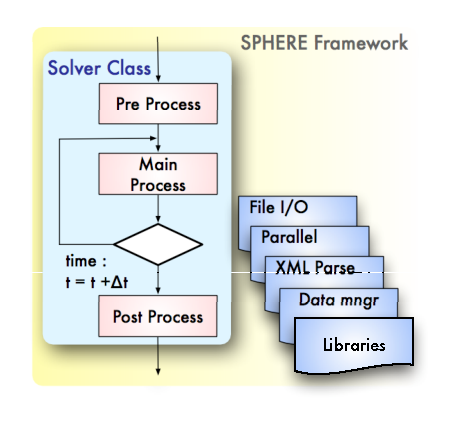
\includegraphics[width=8cm,clip]{Sphere_Control.eps}
\end{center}
\caption{V-Sphereの制御構造.プリ,メイン,ポストの処理プロセスが組み込まれており,提供されるライブラリ機能を用いてソルバークラスを構築します.}
\label{fig:Control structure}
\end{minipage} \hfill
\begin{minipage}{.47\textwidth}
\begin{center}
\includegraphics[width=7.5cm,clip]{DerivedClasses.eps}
\end{center}
\caption{差分プログラミングによるソルバークラスの開発.SklSolverBaseクラスから派生したFlowBaseクラスに共通機能をまとめ,このFBクラスを用いて目的のCBCソルバークラスを作成します.}
\label{fig:DerivedSolvers}
\end{minipage}
\end{figure}


V-Sphereの機能を用いて作成したアプリケーションはソルバークラスとしてV-Sphere自身に登録することができ,登録されたソルバークラス群は共通のユーザインターフェイスを備えたアプリケーションとして振る舞います.
\textbf{図\ref{fig:DerivedSolvers}}に示すようにSklクラス,SklBase\index{SklBase}クラス,およびSklSolverBaseクラスを提供します.
ここでは,SklSolverBaseクラスから流体解析に広く用いられる基本機能を抽出したFlowBaseクラスを作成しています.
ソルバークラスとしては,CBCクラスが派生し,さらにCBCクラスを継承してCPCソルバクラスが派生しています.
また,別の系統としてBCMソルバークラスが作成されています.
これらのソルバークラスは,例えば,シミュレートする物理現象や形状近似度,変数配置などが異なるソルバーですが,FlowBaseクラスにより統一的な振る舞いをします.
つまり,異なるソルバーであっても,ユーザーインターフェイスが統一されたアプリケーションとして構築することができます.

%
\section{CBCソルバークラス}
CBC(Cartesian based, Binary shape representation, Collocated)ソルバークラスは,V-Sphereコンポーネント群とクラスライブラリを利用して実装した非定常非圧縮性流体のソルバークラスです.
ソルバーを構築する上で必要な,パラメータハンドリング,主要な境界条件処理とパラメータの関連づけ,ファイル入出力,並列計算処理,組み込み例題など,コアアルゴリズム以外の部分は,FlowBaseクラスなどにパッケージ化しています.

CBCソルバークラスは,下記のような特徴を持っています.

\begin{description}
\item[ ] 形状近似   :キューブ近似(Binary Voxel)
\item[ ] 変数配置   :コロケート
\item[ ] 離散化    :有限体積法
\item[ ] 時間積分   :一次精度Euler陽解法%,二次精度Adams-Bashforth法,二次精度Crank-Nicolson法
\item[ ] 空間スキーム :一次精度風上,三次精度MUSCL%,二次精度中心,
\item[ ] 解法     :Fractional Step法
\item[ ] 反復法    :Jacobi緩和法, Point SOR, 2-colored SOR-SMA(ストライドメモリアクセス版)
%\item[ ]         2-colored SOR-CMA(連続メモリアクセス版)
\item[ ] スタート機能 :Initial(Impulsive, Smooth), 指定時刻からの再スタート
\item[ ] 入力ファイル :モデルファイル(svx, sbxフォーマット),XMLファイル(計算条件など)
\item[ ] 出力ファイル :sphフォーマット,履歴ファイル,モニター出力
\item[ ] 外部境界条件 :固定・移動壁面,流入,流出,周期,対称,トラクションフリー
\item[ ] 内部境界条件 :壁面,速度規定,流出,部分周期境界,圧力損失,多孔質
\item[ ] 温度境界条件 :断熱,熱伝導,熱伝達,輻射,熱流束,等温
\item[ ] 並列ライブラリ:mpich, mpich2, OpenMPI
\item[ ] 並列化    :等分割,多重連結領域分割
\item[ ] 組込み例題機能:キャビティフロー問題など,基本的な問題
\end{description}





%%%
\chapter{インストール}
\label{chpt:install}
\begin{abstract}
この章では,MPI通信ライブラリ,V-Sphere,CBCソルバークラスのインストールとコンパイルについて説明します.MPI通信ライブラリ,V-Sphereの詳細なインストールについては,V-Sphereユーザガイド(\verb|Vsphere_UG.pdf|)を,CBCソルバークラスの詳細についてはCBCソルバークラス説明書(\verb|Inside_CBC.pdf|)を参照してください.
\end{abstract}
%
%%
\section{MPIライブラリのインストール}
\label{sec:install MPI}

OpenMPI\footnote{http://www.open-mpi.org/}のインストールについて説明します.

\begin{enumerate}
\item autotoolsによるコンパイル\\
autotools~\cite{autotools}を用いて作成されたパッケージは容易にインストールができます.
典型的な場合,インストールまでの全工程が自動化され,ソースコードを展開した後,以下のコマンドを入力するだけで全てが完了します.
{\small
\begin{program}
./configure && make && make install
\end{program}
}

\item シェルスクリプトを用いたコンパイル環境の設定\\
configureのために,次のようなスクリプトを用意して実行します.
インストールディレクトリは\verb|/usr/local/openmpi|とします.
コンパイラは,Intel Compiler icpc/ifortの利用を指定しています.

{\small
\begin{program}
$ cat config_ompi.sh

#!/bin/sh
export CC=icc
export CFLAGS=-O3
export CXX=icpc
export CXXFLAGS=-O3
export F77=ifort
export FFLAGS=-O3
export FC=ifort
export FCFLAGS=-O3
#
./configure --prefix=$1

$ ./config_ompi.sh /usr/local/openmpi
\end{program}
}

\item コンパイルの実行とインストール\\
{\small
\begin{program}
$ make
$ sudo make install
\end{program}
}

\item PATHの設定\\
実行時のmpiexec\footnote{mpirunでも動きます.}が正しいパスになっているかどうかをwhichコマンドで確認します\footnote{Mac OSXの場合には上記のように,デフォルトでインストールされているOpenMPIの方を見に行くので,インストールしたOpenMPIのPATHを最初の方に書いておきます.}.

{\small
\begin{program}
$ which mpiexec
\end{program}
}

\item 環境変数の設定\\
実行時に必要な環境変数をホームディレクトリの\verb|.bash_profile|などに記述しておきます.

{\small
\begin{program}
export LD_LIBRARY_PATH=/usr/local/openmpi/lib:$LD_LIBRARY_PATH
export DYLD_LIBRARY_PATH=/usr/local/openmpi/lib:$DYLD_LIBRARY_PATH
\end{program}
}

\end{enumerate}

%
\section{V-Sphereのインストール}
\label{sec:install vsphere}
V-Sphereのインストールは,MPI通信ライブラリのインストールの後に行います.

%
\subsection{autotoolsを用いたコンパイル環境の設定}
まず,\verb|configure|の設定を行います.
次のスクリプトの例では,インストールディレクトリを\verb|/usr/local/sphere/|に指定しています.
もし,\verb|/usr/local/|領域へのアクセス権限がない場合には,各ユーザが書き込める場所を指定します.
また,LDFLAGSには,コンパイラへの適切なパスを指定します.

{\small
\begin{program}
$ cat configure.sh
$ ./configure --prefix=$1 \
              --with-comp=INTEL \
              --with-ompi=/usr/local/openmpi \
              CC=icc \
              CFLAGS=-O3 \
              CXX=icpc \
              CXXFLAGS=-O3 \
              FC=ifort \
              FCFLAGS=-O3 \
              F90=ifort \
              F90FLAGS=-O3 \
              LDFLAGS=-L/opt/intel/Compiler/11.1/089/lib/intel64
\end{program}
}

上記のインストールシェルは,引数としてインストールディレクトリを指定し,次のように実行します.
この時点で\verb|autotools|のバージョンが違う場合には以下のコマンドをV-Sphereディレクトリで実行し,環境を合わせます.

{\small
\begin{program}
$ aclocal
$ autoconf
$ automake -a
\end{program}
}

\verb|configure|により,利用者の環境を調査し,適切なコンパイル環境を設定します.

{\small
\begin{program}
$ configure.sh /usr/local/sphere
\end{program}
}

%
\subsection{モジュールの作成とインストール}
\verb|configure|の後,次のコマンドを実行します.

{\small
\begin{program}
$ make
$ sudo make install または make install
\end{program}
}

make時に\verb|libimf.so|が見つからないなどのメッセージが出る場合は,ホームディレクトリの\verb|.bash_profile|などにコンパイラのLD\_LIBRARY\_PATHパスを加えておきます.
{\small
\begin{program}
export LD_LIBRARY_PATH=/opt/intel/Compiler/11.1/089/lib:$LD_LIBRARY_PATH
\end{program}
}

%
\subsection{アンインストール}
V-Sphereをアンインストール\index{アンインストール!V-Sphereの@V-Sphereの---}する場合には,インストールしたディレクトリ(configureでオプション指定したディレクトリ:ここでは \verb|/usr/local/sphere|)の\verb|sphere|を削除します.

%
\subsection{倍精度計算モジュール}
単精度計算と倍精度計算では,それぞれ専用のV-Spghereライブラリが必要になり,単精度計算と倍精度計算で異なる精度のモジュールを別々に用意します.
倍精度計算モジュールを生成する場合には,configure時に\verb|--with-real=double|オプションを追加してください.
このオプションは,コンパイルオプションに下記のように\verb|-DREAL_IS_DOUBLE|を追加します.

{\small
\begin{program}
CFLAGS         : -O3 -DREAL_IS_DOUBLE
CXXFLAGS       : -O3 -DREAL_IS_DOUBLE
\end{program}
}

両方必要になる場合には,両方のV-Sphereライブラリを用意しておき,CBCソルバークラスのコンパイル時にリンク先を変更して,コンパイルします.


%%
\hypertarget{tgt:installCBC}{\section{CBCソルバークラスのインストールとコンパイル}}
\label{sec:install CBC}

本節では,ソルバークラスのインストールについて説明します.
提供されるソルバークラスのアーカイブ\verb|CBC_x.x.x.tar.gz|は,ソルバークラスのソースコードです\footnote{CBC\_x.x.x.tar.gzのx.x.xにはリリースバージョン番号が入ります.}.

%%
\subsection{アーカイブの解凍}
{\small
\begin{program}
$ tar xvfz CBC_x.x.x.tar.gz
\end{program}
}

解凍すると,以下のようなファイル構成になります\footnote{doxygenディレクトリについては,doxygenファイルを生成するために必要な設定ファイルのみを提供しています.Confディレクトリ内でmakeを実行すると各ディレクトリにdoxygenファイルが生成されます.}.

{ \small
\begin{program}
CBC_x.x.x
  |
  +- BUILD                        アプリケーションのコンパイル方法のメモ
  +- COPYING                      コピーライト
  +- README                       最初に見るべきファイル
  +- RELEASE                      リリース情報
  |
  +- doc                          ドキュメント
  |   +- cbc_ug.pdf               CBCソルバークラスのユーザガイド
  |   +- vsphere_ug.pdf           V-Sphereのユーザーガイド
  |   +- cbc_examples.pdf         検証の例題集
  |
  +- doxygen                      Doxygenドキュメントディレクトリ
  |   +- CBC                      CBCクラスのドキュメント
  |   +- Conf                     Doxygenファイルを生成するための設定ファイル
  |   +- FB                       FBクラスのドキュメント
  |   +- IP                       Intrinsicクラスのドキュメント
  |
  +- example                      例題
  |   +- 3Dcavity                 三次元のキャビティフロー(立方体領域)
  |   +- LDC112                   辺長1:1:2のキャビティフロー
  |   +- dragon                   ドラゴン形状周りの流れ
  |   +- Duct3D                   管路内流れ
  |   |   +- inner                ドライバ周期境界指定
  |   |   +- outer                外部周期境界指定
  |   +- PMT                      性能測定用パラメータ群
  |   +- SHC1D                    定常1次元熱伝導
  |
  +- src                          ソースコード
  |   +  F_CBC                    CBCクラスのFortranファイル
  |   +- F_CPC                    CPCクラスのFortranファイル
  |   +- F_VOF                    VOFクラスのFortranファイル
  |   +- FB                       FlowBaseクラス(ユーザー定義クラス群)
  |   +- IP                       組み込み例題クラス群
  |   +- PRJ_CBC	                 CBCプロジェクト
  |      +- app                  アプリケーションコンパイルディレクトリ
  |         ...                  他ソースファイル
  |         Makefile
  |      +- bin                  バイナリモジュール格納ディレクトリ
  |      +- CBC                  CBCソルバークラスのソースファイル
  |      |   +- CBC.xml          CBCクラスのコンパイル環境設定
  |      |      ...              他ソースファイル
  |      |      Makefile
  |      +- FB                   非ソルバークラスディレクトリ FlowBase
  |      |   +- FB.xml           FBクラスのコンパイル環境設定  
  |      |      Makefile
  |      +- IP                   非ソルバークラスディレクトリ 組み込み例題クラス群
  |      |   +- IP.xml           IPクラスのコンパイル環境設定 
  |      |      Makefile
  |      +- Makefile             アプリケーションコンパイル用 Linux/Mac
  |         PRJ_CBC.xml          CBCのコンパイル設定
  +- xsd
     CBC_xxx_FB_xxx.xsd          V-Xpitを用いたパラメータ入力の構造定義ファイル
\end{program}
}
%  |   +- Inside_CBC.pdf           CBCソルバークラスの説明書

%
\subsection{sphPrjToolを用いた簡単なインストールとコンパイル}
既に,並列ライブラリとV-Sphereが正しくインストールされていることを確認します.

まず,sphPrjToolを利用するため,環境変数\verb|SPHEREDIR|を設定します.
下記で\verb|INSTALL_DIR|はV-Sphereのインストールディレクトリを指定します.
次に,\verb|src/PRJ_CBC|ディレクトリで引数にファイル名を渡してsphPrjToolを起動し,プロジェクトのコンパイル設定を利用環境に合わせて再構築します.
localsettingsオプションを指定してresetコマンドを実行すると,sphereライブラリの\verb|config/sph-cfg.xml|に記録されているコンパイル環境情報を元にして,プロジェクト環境情報\verb|PRJ_CBC.xml|を再設定します.

{\small
\begin{program}
$ export SPHEREDIR=INSTALL_DIR
$ cd src/PRJ_CBC
$ sphPrjTool PRJ_CBC.xml
sphPrjTool> reset localsettings
sphPrjTool> print
sphPrjTool> save
sphPrjTool> quit
\end{program}
}

上記の設定の後,コンパイルを行う.

{\small
\begin{program}
$ make
\end{program}
}

%
\subsection{アンインストール}
アンインストール\index{アンインストール!SolverClassの@SolverClassの---}は,SolverClassのディレクトリごと削除します.

%
\subsection{並列計算モジュールのコンパイル}
V-Sphereは逐次計算のモジュールと並列計算のモジュールは異なるので,コンパイル時にオプションで切り替えます.
並列計算\index{へいれつけいさん@並列計算}をする場合は,\verb|PRJ_CBC.xml|内に下記の記述を追加するか,sphPrjToolを用いて設定を変更します.
デフォルトでは逐次実行モジュールになっています.

{\small
\begin{program}
$ sphPrjTool PRJ_CBC.xml
sphPrjTool> module parallel
sphPrjTool> print
sphPrjTool> save
sphPrjTool> quit
\end{program}
}

%
\hypertarget{tgt:win_compile}{\subsection{Windowsでのコンパイルと実行}}

%
\subsubsection{プロジェクトの作成}
プロジェクトツール\footnote{C:{\yen}Program Files{\yen}sphere{\yen}bin{\yen}sphPrjTool.exe}を用いWindows用のプロジェクトを作成します.
プロジェクトツールの使用については,V-Sphere\_ug.pdfを参照してください.
プロジェクトツールによって以下のMakefileが生成されます.
提供ファイルのlibxml2, zlib, iconvのインストールパスは\lq\lq C:{\yen}Program Files{\yen}ext\_libs{\yen}\rq\rq 配下になっているので注意してください.

{\small
\begin{program}
PRJ_CBC
  ├─ Makefile.win
  ├─ project_local_settings
  ├─ CBC
  │    └─ Makefile.win
  ├─ FB
  │    └─ Makefile.win
  └─ IP
       └─ Makefile.win
\end{program}
}

%
\subsubsection{コンパイル}
作成した\verb|Makefile.win|を用いてmakeを行います.
コマンドプロンプトから行うが,Visual Studioの\verb|nmake.exe|を使用するので「Visual Studio 2008 コマンド プロンプト」を起動して行います.
「Visual Studio 2008 コマンド プロンプト」は「Visual Studio 2008」―「Visual Studio Tools」メニューの配下にあります.

以下,nmakeによるコンパイルコマンドです.

{\small
\begin{program}
nmake -f Makefile.win
\end{program}
}

%
\subsubsection{CBCの実行}
ソルバの実行は必ずローカルディスクにて実行します.
ネットワークパス(ネットワークドライブ)で行うとエラーとなります\footnote{現時点 \today では原因不明です.}.

以下の設定を行います.
\begin{enumerate}
\item MPICH2のbinフォルダへパスの追加\\
並列実行ではエラーとなりませんが,逐次実行にてエラーとなります.

\item Windowsファイアウォール設定
\verb|sphere.exe|を例外へ追加します.
コントロールパネル-Windowsセキュリティセンター - Windowsファイアウォール-例外に実行を行う\verb|sphere.exe|を登録します.
\end{enumerate}


\paragraph{逐次実行方法}
次のように実行します.


{\small
\begin{program}
$ set PATH=%PATH%;C:\Program Files\MPICH2\bin
$ pwd
D:\work\CBC-1.3.0\example\3Dcavity
$ ..\..\src\PRJ_CBC\bin\sphere.exe cavity.xml
\end{program}
}


\paragraph{並列実行方法:ローカルホストにて実行}
複数のホストマシンにて実行する方法は,V-Sphere ユーザマニュアル「V-SphereUG.pdf」-11. Windows 対応(使用者向け)又はMPICH2のマニュアルを参照してください.

{\small
\begin{program}
$ pwd
D:\work\CBC-1.3.0\example\3Dcavity
$ "C:\Program Files\MPICH2\bin\mpiexec.exe" -np 4 ..\..\src\PRJ_CBC\bin\sphere.exe cavity.xml
\end{program}
}


%%
\hypertarget{tgt:win_opmi_binary}{\subsection{OpenMPIバイナリパッケージを用いたコンパイルと実行}}
OpenMPI 1.5.3よりWindowsバイナリーパッケージ\footnote{OpenMPI\_v1.5.3-2\_win32.exe}が提供されています.
OpenMPIを以下のフォルダにインストールしたと仮定して説明します.
{\small
\begin{program}
	C:\Program Files\OpenMPI
\end{program}
}

%
\paragraph{V-Sphereのコンパイル}
Config.winを変更します($\ll$で示す\verb|MPICH_DIR, MPICH_LIBS, MPICH_CFLAGS|).

{\small
\begin{program}
#
# SPHERE - Skeleton for PHysical and Engineering REsearch
#
# Copyright (c) RIKEN, Japan. All right reserved. 2004-2011
#
#

# folder settings
SPHEREDIR=C:\Program Files\sphere
INTELCXX_DIR=C:\Program Files\Intel\Compiler\C++\10.1.021\IA32
INTELFC_DIR=C:\Program Files\Intel\Compiler\Fortran\10.1.021\IA32
MSSDKS_DIR=C:\Program Files\Microsoft SDKs\Windows\v6.0A
MSVS_DIR=C:\Program Files\Microsoft Visual Studio 9.0
MPICH_DIR=C:\Program Files\OpenMPI <<

EXTLIBS_PATH=C:\Program Files\ext_libs
LIBXML2_DIR=$(EXTLIBS_PATH)\libxml2
ZLIB_DIR=$(EXTLIBS_PATH)\zlib
ICONV_DIR=$(EXTLIBS_PATH)\iconv

# flags ssettings
CFLAGS=/O3 /Qprec-div- /c /TP /MT /DWIN32 /D_WIN32 /DSKL_TIME_MEASURED /D_CATCH_BAD_ALLOC
#CXXFLAGS=/fast /c /TP /MD /DWIN32 /D_WIN32
#CXXFLAGS=/O3 /c /TP /MD /DWIN32 /D_WIN32
#CXXFLAGS=/O3 /Qipo /c /TP /MD /DWIN32 /D_WIN32
#CXXFLAGS=/O3 /Qprec-div- /c /TP /MD /DWIN32 /D_WIN32
CXXFLAGS=/O3 /Qprec-div- /c /TP /MT /DWIN32 /D_WIN32 /DSKL_TIME_MEASURED/D_CATCH_BAD_ALLOC
FCFLAGS=/O3 /Qprec-div- /c /TP /MT /DWIN32 /D_WIN32 /DSKL_TIME_MEASURED
F90FLAGS=/O3 /Qprec-div- /c /TP /MT /DWIN32 /D_WIN32 /DSKL_TIME_MEASURED

# libs settings
MPICH_LIBS= libmpi.lib <<
#XML2LIBS=libxml2.lib zlib.lib libm.lib ws2_32.lib
XML2LIBS=libxml2.lib zdll.lib libmmt.lib ws2_32.lib

# include libpath settings
INCLUDES = \
			/I"$(TOP_BUILDDIR)\include" \
			/I"$(LIBXML2_DIR)\include" \
			/I"$(ZLIB_DIR)\include" \
			/I"$(ICONV_DIR)\include"

LDFLAGS = \
		/LIBPATH:"$(INTELCXX_DIR)\lib" \
		/LIBPATH:"$(LIBXML2_DIR)\lib" \
		/LIBPATH:"$(ZLIB_DIR)\lib" \
		/LIBPATH:"$(ICONV_DIR)\lib"

MPICH_CFLAGS=/I"$(MPICH_DIR)\include" /DOMPI_IMPORTS <<
MPICH_LDFLAGS=/LIBPATH:"$(MPICH_DIR)\lib"

# exec settings
CC="$(INTELCXX_DIR)\bin\icl.exe"
CXX="$(INTELCXX_DIR)\bin\icl.exe"
FC="$(INTELFC_DIR)\bin\ifort.exe"
F90="$(INTELFC_DIR)\bin\ifort.exe"
AR="$(INTELCXX_DIR)\bin\xilib.exe"
LINK="$(INTELCXX_DIR)\bin\xilink.exe"
MANF_TOOL=mt.exe
CP=copy
RM=del /F /Q

# environments
PATH=$(MSVS_DIR)\Common7\IDE;$(MSVS_DIR)\VC\bin;$(MSSDKS_DIR)\bin;$(PATH);
INCLUDE=$(MSVS_DIR)\VC\INCLUDE;$(MSSDKS_DIR)\include;$(INCLUDE)
LIB=$(MSVS_DIR)\VC\LIB;$(MSSDKS_DIR)\lib;$(LIB)
LIBPATH=$(MSVS_DIR)\VC\LIB;$(LIBPATH)

\end{program}
}


\begin{enumerate}
\item OpenMPIのインストールパスの変更
\item \verb|libmpi.lib|の変更
\item OMPI\_IMPORTSマクロの追加
\end{enumerate}

V-Sphereをコンパイルし,作成したライブラリとインクルードファイルをC:{\yen}program files{\yen}sphere\_ompiに配置します.

{\small
\begin{program}
$ nmake /f Makefile.win
\end{program}
}

%
\paragraph{ソルバCBCのコンパイル}
\verb|project_local_settings|を変更します.\\
\verb|SPHEREDIR, MPICH_DIR, MPICH_CFLAGS, MPICH_LDFLAGS, MPICH_LIBS, SPHERE_CFLAGS, SPHERE_LDFLAGS|

{\small
\begin{program}
#
# SPHERE - Skeleton for PHysical and Engineering REsearch
#
# Copyright (c) RIKEN, Japan. All right reserved. 2004-2010
#
#
CC=gcc
CFLAGS=-g -O2
CXX="C:\Program Files\Intel\Compiler\C++\10.1.021\IA32\Bin\icl.exe"
CXXFLAGS=/O3 /Qipo /Qprec-div-
FC=f95
FCFLAGS=-g -O2
F90="C:\Program Files\Intel\Compiler\Fortran\10.1.021\IA32\Bin\ifort.exe"
F90FLAGS=/O3 /Qipo /Qprec-div-
LDFLAGS=/LIBPATH:"C:\Program Files\Intel\Compiler\Fortran\10.1.021\IA32\Lib"
LIBS=ws2_32.lib libifport.lib libmmt.lib libifcoremt.lib
SPH_USR_DEF_LIBS=
UDEF_OPT=-DNON_POLYLIB -DNON_CUTLIB
UDEF_INC_PATH=
UDEF_LIB_PATH=
UDEF_LIB_UPPER=
UDEF_LIB_LOWER=
SPHEREDIR=C:\Program Files\sphere_ompi <<
SPH_DEVICE=IA32_WIN
MPICH_DIR=C:\Program Files\OpenMPI <<
MPICH_CFLAGS=/I"C:\Program Files\OpenMPI\include" <<
MPICH_LDFLAGS=/LIBPATH:"C:\Program Files\OpenMPI\lib" <<
MPICH_LIBS=libmpi.lib <<
XML2FLAGS=/I"C:\Program Files\ext_libs\libxml2\include" /I"C:\Program Files\ext_libs\iconv\include"
XML2LIBS=libxml2.lib zdll.lib
SPHERE_CFLAGS=/DSKL_TIME_MEASURED /D_CATCH_BAD_ALLOC /I"C:\Program Files\sphere_ompi\include" <<
SPHERE_LDFLAGS=/LIBPATH:"C:\Program Files\sphere_ompi\lib" <<
SPHERE_LIBS=libsphapp.lib libsphbase.lib libsphfio.lib libsphdc.lib libsphcrd.lib libsphcfg.lib 
            libsphftt.lib libsphvcar.lib
REALOPT=
CXXFLAGS_DEF=/c /TP /MT /DWIN32 /D_WIN32
F90FLAGS_DEF=/c /MT
SPHERE_DEFINE=/DSKL_TIME_MEASURED /D_CATCH_BAD_ALLOC
ZLIB_DIR=C:\Program Files\ext_libs\zlib
ZLIB_LDFLAGS=/LIBPATH:"C:\Program Files\ext_libs\zlib\lib"
INTELCXX_DIR=
INTELF90_DIR=
LIBXML2_DIR=C:\Program Files\ext_libs\libxml2
MSSDKS_DIR=C:\Program Files\Microsoft SDKs\Windows\v6.0A
MSVS_DIR=C:\Program Files\Microsoft Visual Studio 9.0
INTELCXXBIN_DIR=C:\Program Files\Intel\Compiler\C++\10.1.021\IA32\Bin
INTELF90BIN_DIR=C:\Program Files\Intel\Compiler\Fortran\10.1.021\IA32\Bin
INTELCXXLIB_DIR=C:\Program Files\Intel\Compiler\C++\10.1.021\IA32\lib
INTELF90LIB_DIR=C:\Program Files\Intel\Compiler\Fortran\10.1.021\IA32\Lib
ICONV_DIR=C:\Program Files\ext_libs\iconv
XML2LDFLAGS=/LIBPATH:"C:\Program Files\ext_libs\libxml2\lib" 
            /LIBPATH:"C:\Program Files\ext_libs\iconv\lib"
SPH_EXTERNAL_HEADER_PATH=/I..\..\Cutlib_2_0_0\include /I..\..\FB /I..\..\F_CBC /I..\..\IP 
                         /I..\..\Polylib_2_0_2\include 
SPH_PARA_MODULE=MPI
\end{program}
}


\begin{enumerate}
\item OpenMPI用のV-Sphereのパスの変更
\item OpenMPIのインストールパスの変更
\item \verb|libmpi.lib|の変更
\end{enumerate}

ソルバCBCをコンパイルします.
{\small
\begin{program}
$ pwd
D:\work\CBC-1.3.0\src\PRJ_CBC
$ nmake -f Makefile.win
\end{program}
}

%
\paragraph{ソルバCBCの実行}
\verb|sphere.exe|を実行する前にOpenMPIへのパスを追加します.

{\small
\begin{program}
$ set PATH=%PATH%;C:\Program Files\OpenMPI\bin
\end{program}
}

ローカルホストにて,\verb|mpirun.exe|により並列実行を行います\footnote{逐次実行はエラーとなっています.}.
{\small
\begin{program}
$ pwd
D:\work\CBC-1.3.0\example\3Dcavity
$ "C:\Program Files\OpenMPI\bin\mpirun.exe" -np 4  ..\..\src\PRJ_CBC\bin\sphere.exe cavity.xml
\end{program}
}





%%%
\chapter{基礎方程式と解析方法}
\label{chpt:eqs}
\begin{abstract}
本章では,CBCソルバークラスが扱う流体の基礎方程式について簡単に説明します.詳細はCBCソルバークラス説明書(\verb|Inside_CBC.pdf|)を参照してください.
\end{abstract}
%
\include{CBC_Eqs}



%%%
\chapter{解析モデルの作成}
\label{chpt:model}
\begin{abstract}
この章では,解析モデルの作成方法を説明します.解析モデルの作成については,2種類の方法があります.まず最初にSTLやOBJなどのフォーマットの形状データを基に,ボクセル作成アプリケーションV-Xgenで行う解析モデルの作成法について説明します.次に,組み込み例題を用いたモデルの扱いについて説明します.
\end{abstract}
%

\graphicspath{{./fig_Model/}}

%
\section{形状近似度による解析モデルの分類}
\label{sec:classification of model}
直交格子を用いる流体解析では,解析対象となる形状を直交格子上でどのように扱うかにより,計算のロバスト性,予測精度,計算時間,計算格子(解析モデル)の作りやすさなどの特性が異なります.一般には,\textbf{図\ref{fig:class model}}のように分類することができます\cite{CFDハンドブック:03}.

\begin{figure}[htdp]
\begin{center}
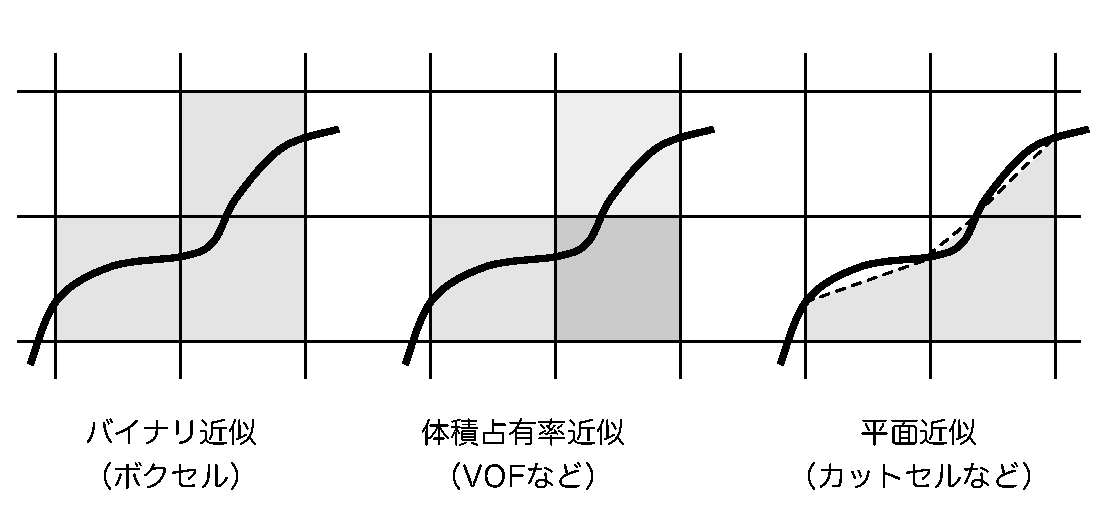
\includegraphics[width=11cm,clip]{classification.eps}
\caption{直交格子における形状近似度の分類}
\label{fig:class model}
\end{center}
\end{figure}

%
\subsection{Binary Voxel}
\label{sec:binary voxel}
Binary Voxel\index{Binary Voxel}モデルは,\textbf{図\ref{fig:Eport binary voxel}}に示すように立方体のセル要素単位で形状を表現する解析モデルです.
物体の形状近似としては最も簡単であり,モデル作成時のロバスト性に大きな利点があります.

\begin{figure}[htbp]
\begin{minipage}{.6\textwidth}
\begin{center}
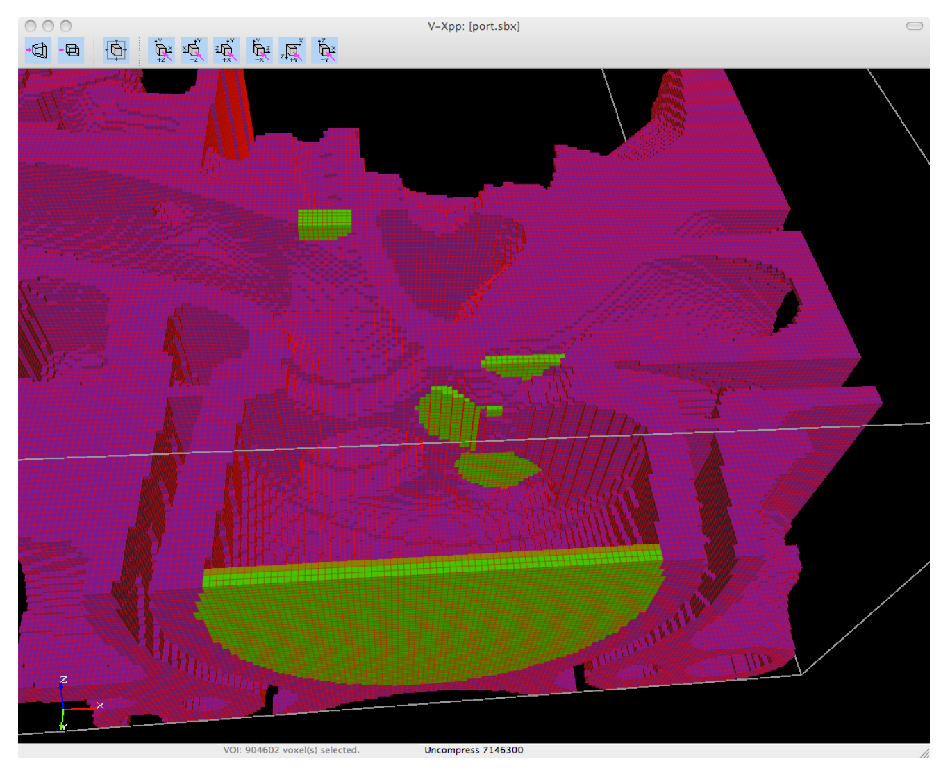
\includegraphics[width=8cm,clip]{eport.eps}
\end{center}
\caption{バイナリボクセルによる機械部品の形状表現とセルID設定}
\label{fig:Eport binary voxel}
\end{minipage} \hfill
\begin{minipage}{.38\textwidth}
\begin{center}
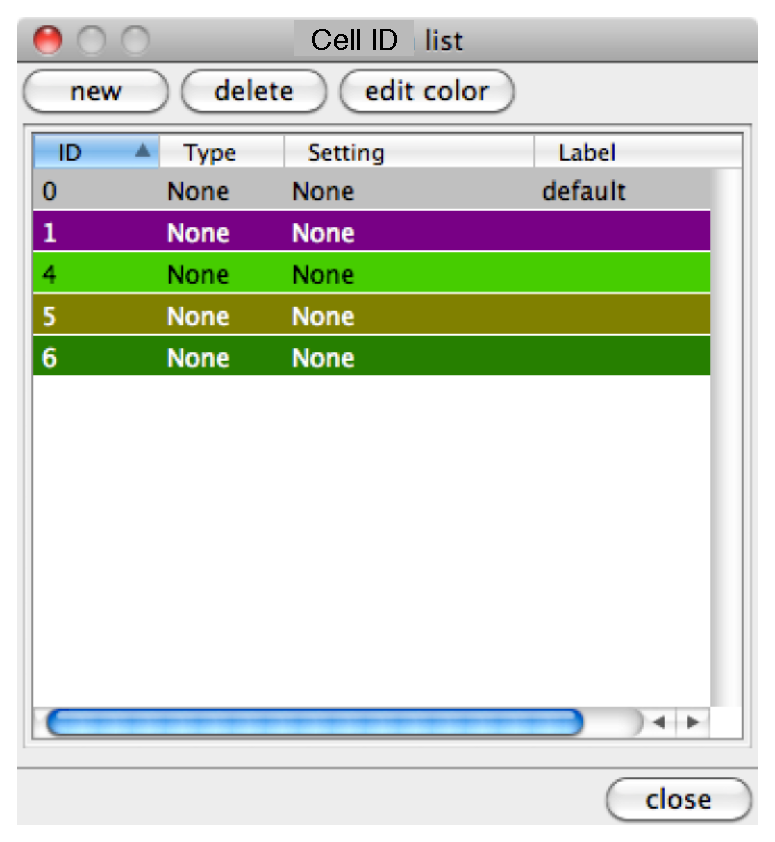
\includegraphics[width=6cm,clip]{Mlist.eps}
\end{center}
\caption{V-XgenでのセルID設定リスト}
\label{fig:ID set on V-Xgen}
\end{minipage}
\end{figure}

%
\subsection{体積率モデル}
Binary Voxelの形状近似度を改善する方法の一つで,セル内における流体の占有率を考慮した計算をする場合に利用します.
陽的な面の情報をもたないので,界面は拡散的に表現される傾向です.補助的に面における開口率を用いる場合には,有限体積法との親和性が高く保存性が改善されます.
%
\subsection{カットモデル}
\label{sec:planar cut}
Binary Voxelでは形状が階段状に近似されるため,計算精度が不足する場合があります.そこで,形状を区分的にカットされた平面として近似するモデルを用います.
CPCソルバー\footnote{\today 未実装.}では,物理量の定義点から物体までの距離情報を用いることにより,ロバスト性と精度向上の両立を図っています.通常のボクセルについてはバイナリボクセルと同様です.


%
\section{セルIDによる境界条件の指定}
\label{sec:ID connection}

CBC/CPCソルバーでは,ボクセルの各セルにIDを与え,このセルIDとパラメータファイルに記述された境界条件情報から,境界条件を設定するしくみになっています.
例えば,ボクセルモデルのセルIDとXML記述のパラメータファイル中では,次のように媒質IDと結びつけられます.

{\small
\begin{program}
<Elem name="Model_Setting">
  <Param name="fluid" id="1"   dtype="INT" value="100" comment="air"/>
  <Param name="solid" id="600" dtype="INT" value="600" comment="wall"/>
  <Param name="solid" id="610" dtype="INT" value="600" comment="piston_head"/>
</Elem>
\end{program}
}

\noindent ここでは,流体であるセルID=1は媒質ID=100によりその物性値が定義され,airのコメントがつけられています.
参照される媒質IDは,Medium\_Tableタグによって次のように指定されます.

{\small
\begin{program}
<Medium_Table>
  <Elem name="Fluid" id="100" comment="Air">
    <Param name="density"              dtype="REAL" value="1.1763" />
    <Param name="specific_heat"        dtype="REAL" value="1007" />
    <Param name="thermal_conductivity" dtype="REAL" value="2.614e-02" />
    <Param name="kinematic_viscosity"  dtype="REAL" value="15.83e-06" />
    <Param name="viscosity"            dtype="REAL" value="18.62e-06" />
    <Param name="sound_of_speed"       dtype="REAL" value="340.0" />
  </Elem>
  <Elem name="Solid" id="600" comment="Fe">
    <Param name="density"              dtype="REAL" value="7870.0" />
    <Param name="specific_heat"        dtype="REAL" value="442.0" />
    <Param name="thermal_conductivity" dtype="REAL" value="80.3" />
  </Elem>
</Medium_Table>
\end{program}
}

媒質IDの指定についての詳細は,\hyperlink{tgt:medium_table}{Medium\_Table}セクションを参照してください.

\pagebreak
%
\section{形状データからの解析モデルの作成手順}
\label{sec:modeling procedure}
V-Xgen\index{V-Xgen}を用いた解析モデル作成の手順を簡単に示します.操作の詳細は,V-Xgenユーザーガイド,およびチュートリアルを参照してください.

\begin{enumerate}
\item V-Xgenの起動\\
アイコンのダブルクリック,または下記のようにコマンドラインからアプリケーションを起動します.

{\small
\begin{program}
$ Vxgen.sh または Vxgen
\end{program}
}

\item ファイルの読み込み\\
入力となる幾何形状STLファイル\index{STL}を読み込みます.
\verb|File > Import > Shape (obj/stl) data files...|のコマンドを実行し,ファイルリストから幾何形状ファイルを選択しロードすると,\textbf{図\ref{fig:V-Xgen mesh}}のように形状モデルが描画されます.\\

\begin{figure}[htbp]
\begin{minipage}{.6\textwidth}
\begin{center}
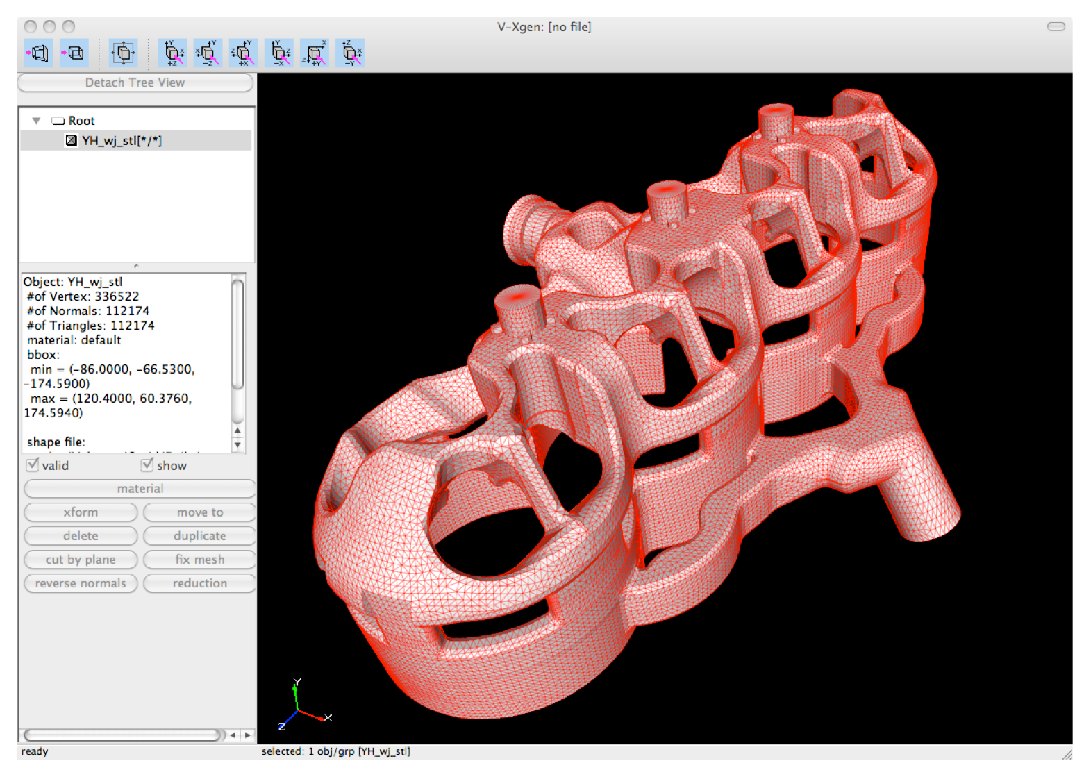
\includegraphics[width=8.5cm,clip]{WJ_mesh.eps}
\end{center}
\caption{V-Xgenでのファイル読み込み}
\label{fig:V-Xgen mesh}
\end{minipage} \hfill
\begin{minipage}{.38\textwidth}
\begin{center}
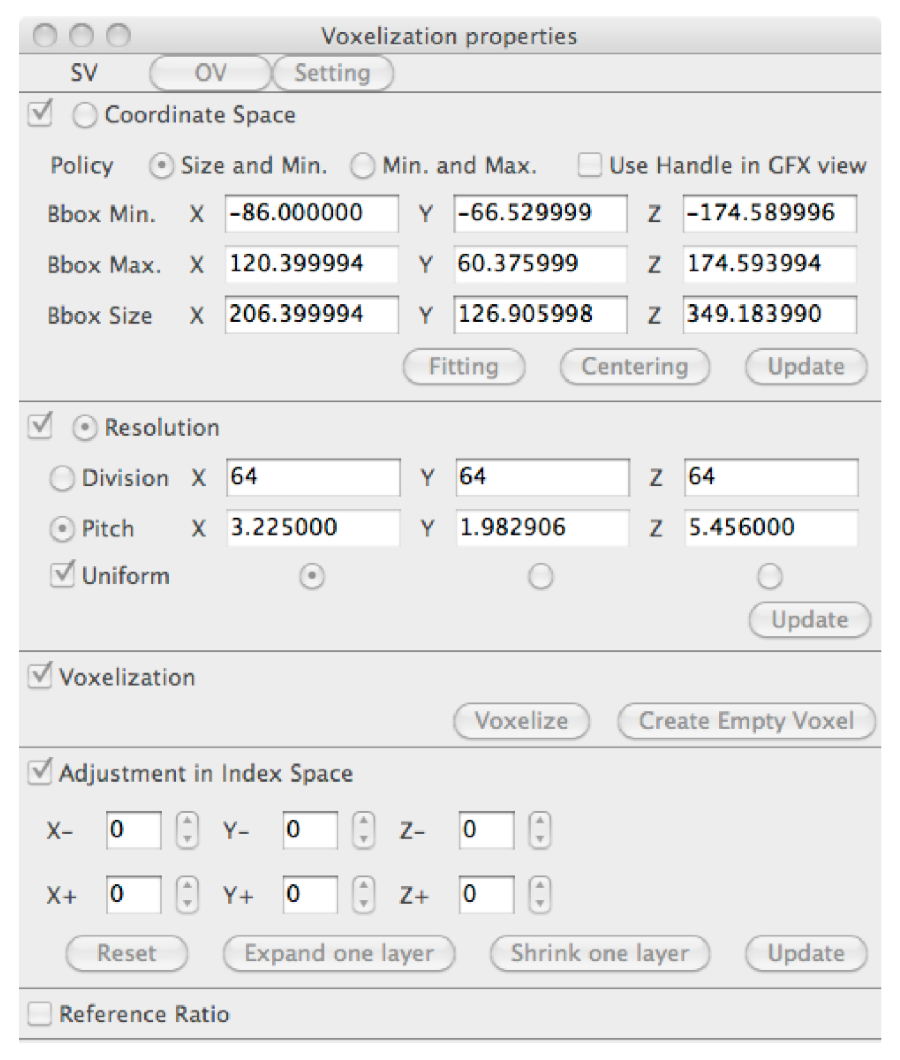
\includegraphics[width=6cm,clip]{SV_dialog.eps}
\end{center}
\caption{ボクセル作成のパラメータ設定ダイアログ}
\label{fig:SV menue}
\end{minipage}
\end{figure}

\item バイナリボクセルの作成\\
\verb|Voxelization > Simple Voxel(SV) ...|を実行すると,\textbf{図\ref{fig:SV menue}}のような直交等間隔ボクセルを作成するダイアログが表示されます.
パラメータを適切に設定して,ボクセルを作成すると,\textbf{図\ref{fig:V-Xgen voxelize}}のようなボクセルのバウンディングボックスが表示されます.
ここで作成するボクセルモデルの範囲は,\textbf{図\ref{fig:cal. region}}に示す計算領域の部分です.
計算に必要な計算領域の外部に位置する仮想セル領域の媒質はXMLパラメータファイルのOuterBoundary$\to$Face\_BC中のCell\_IDタグで指定します.\\

\begin{figure}[htbp]
\begin{minipage}{.48\textwidth}
\begin{center}
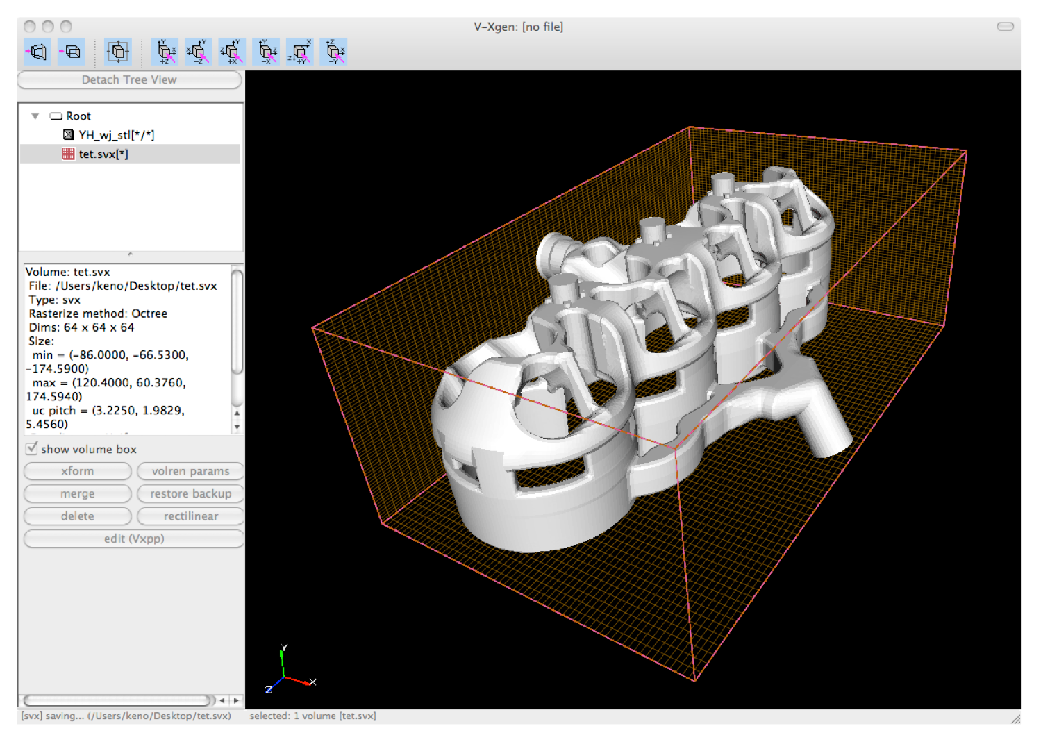
\includegraphics[width=8cm,clip]{voxelize.eps}
\end{center}
\caption{V-Xgenでのボクセル生成}
\label{fig:V-Xgen voxelize}
\end{minipage} \hfill
\begin{minipage}{.48\textwidth}
\begin{center}
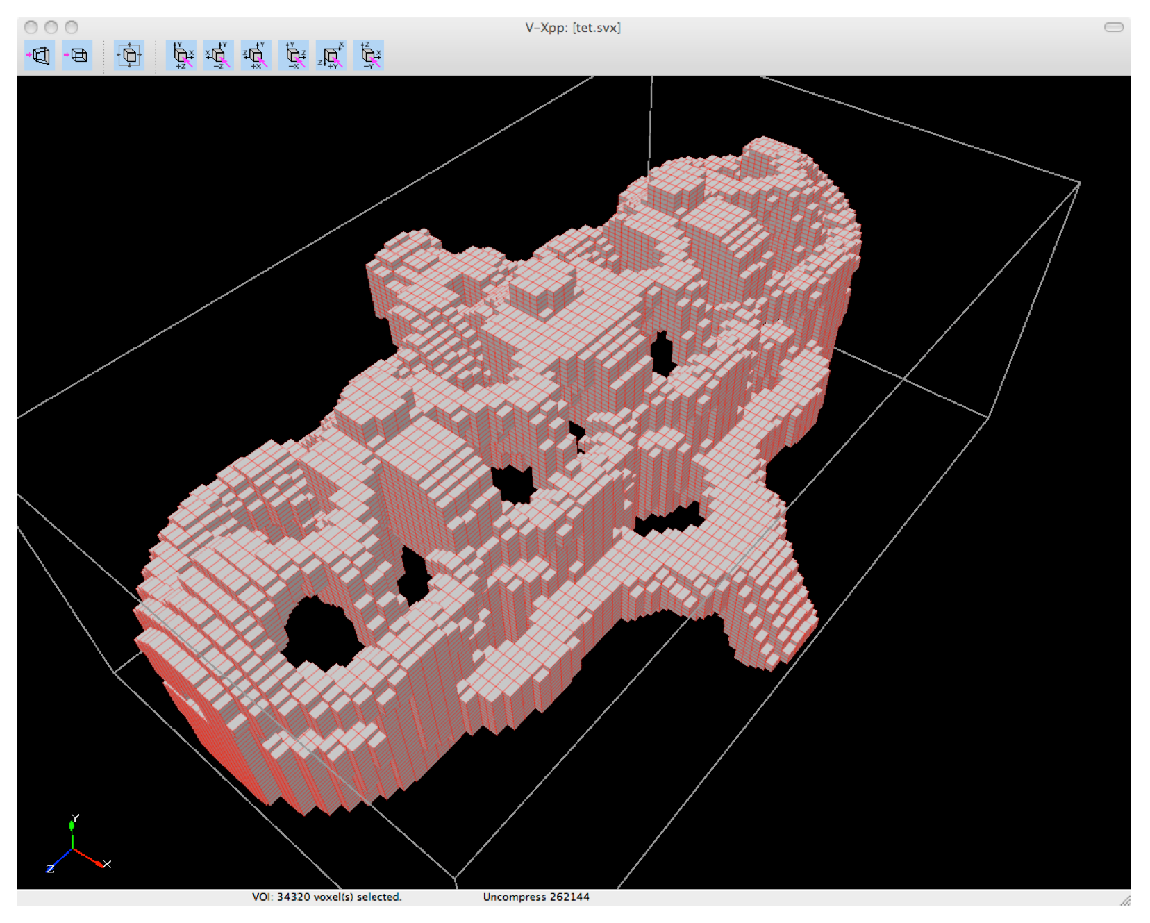
\includegraphics[width=7cm,clip]{WJ_voxel.eps}
\end{center}
\caption{ボクセルモデル.V-XppのVOIコマンドによる選択状態の表示}
\label{fig:V-Xpp voxel}
\end{minipage}
\end{figure}

\begin{figure}[htdp]
\begin{center}
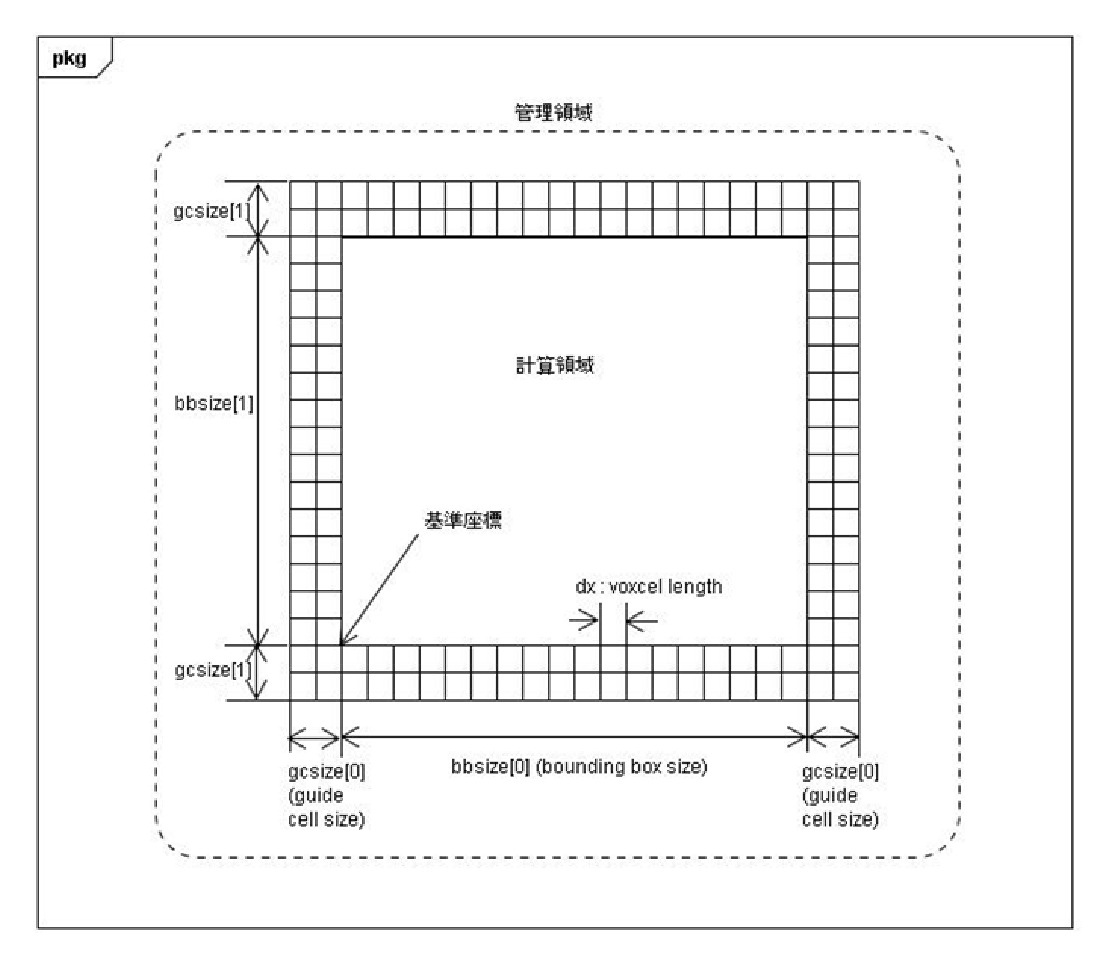
\includegraphics[width=12cm,clip]{clip006.eps}
\caption{計算領域とガイドセル領域の定義}
\label{fig:cal. region}
\end{center}
\end{figure}


\item セルIDの設定\\
V-Xgenで作成したボクセルモデルファイルを,アプリケーションV-Xpp\index{V-Xpp}を用いてセルIDを編集します\footnote{次のバージョンでは,V-Xppの機能をV-Xgenに統合予定です.}.V-Xppを起動し,\verb|File > Open...|を実行してボクセルモデルファイル(*.svx, *.sbx, *.ovx)を選択しロードすると,\textbf{図\ref{fig:V-Xpp voxel}}のようにボクセライズされた形状データが表示されます.\\

 次に,\verb|Volume > Medium List...|を選択し,\textbf{図\ref{fig:V-Xpp Medium list}}に示すセルIDリストを編集します.
ボクセルモデルを\verb|VOI > Select VOI...|や\verb|VOI > Slice Control...|によりボクセルを選択,\verb|VOI > Set Cell ID...|コマンド(\textbf{図\ref{fig:V-Xpp set cell ID}})によりセルIDを選択対象セルに設定します.
セルIDを編集したボクセルモデルは\textbf{図\ref{fig:editted voxel}}のようになるのでファイルに保存します.
ここで,約束事として,\textbf{セルID=0は予約番号でユーザは設定しないこと}に注意してください.\\

また,利用できるIDの設定数に関しては,\hyperlink{tgt:innerboundary}{InnerBoundary}で説明していますが,\textbf{指定できる内部境界条件の数は30個が上限で,かつ指定境界条件数と媒質数の和は63個以下}となる点に注意してください.

\begin{figure}[htbp]
\begin{minipage}{.48\textwidth}
\begin{center}
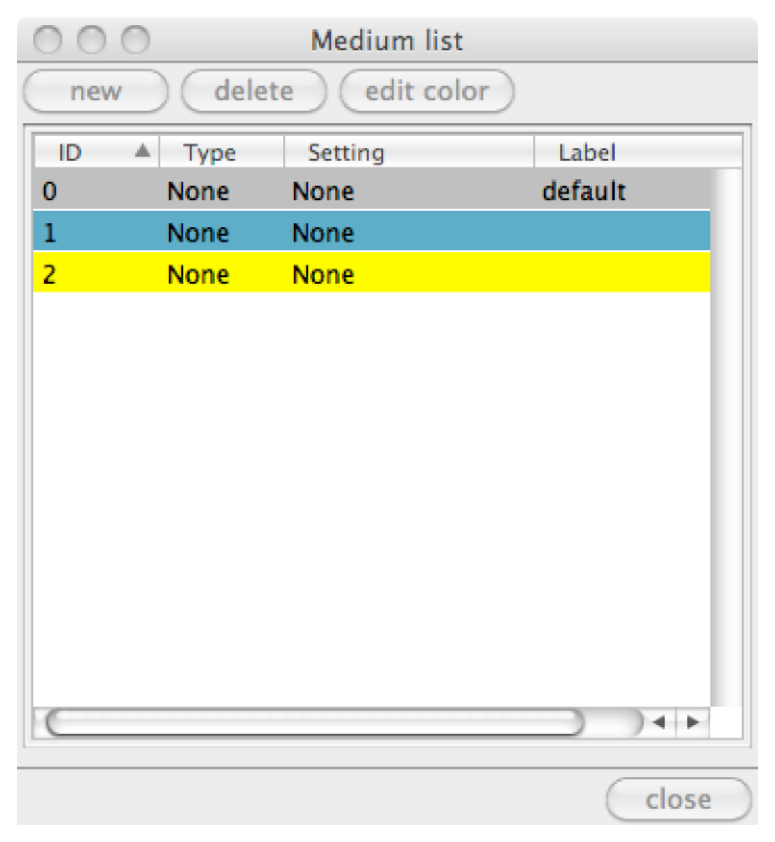
\includegraphics[width=6cm,clip]{VXpp_Mlist.eps}
\end{center}
\caption{セルID編集ダイアログ}
\label{fig:V-Xpp Medium list}
\end{minipage} \hfill
\begin{minipage}{.48\textwidth}
\begin{center}
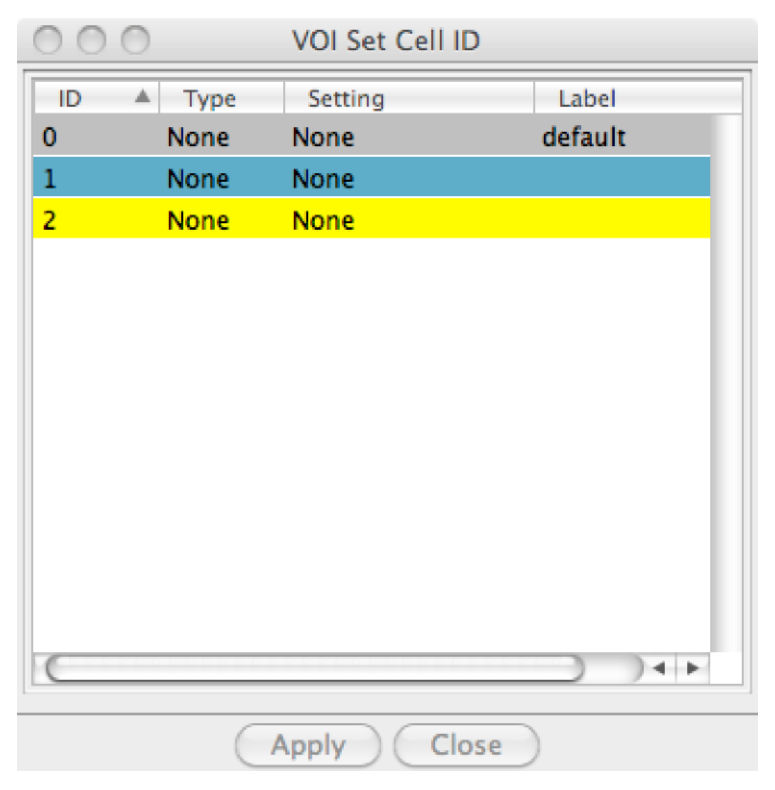
\includegraphics[width=6cm,clip]{VXpp_setID.eps}
\end{center}
\caption{セルID設定ダイアログ}
\label{fig:V-Xpp set cell ID}
\end{minipage}
\end{figure}

\begin{figure}[htdp]
\begin{center}
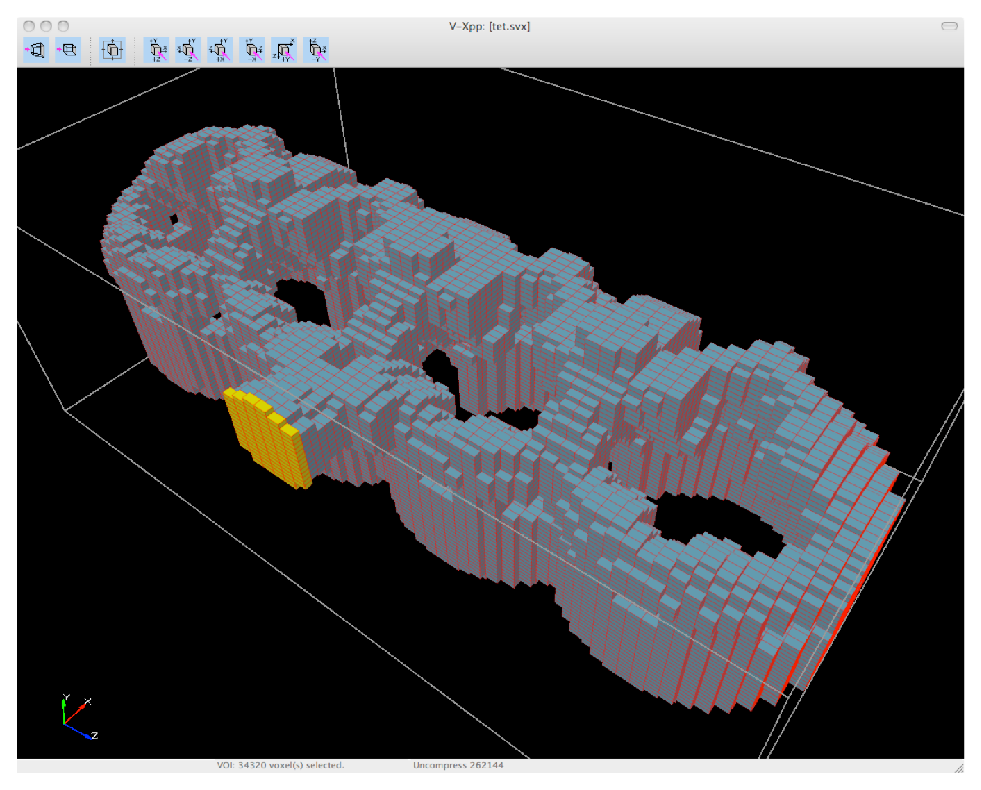
\includegraphics[width=12cm,clip]{VXpp_coloredVoxel.eps}
\caption{V-XppでセルIDを編集したボクセルモデル}
\label{fig:editted voxel}
\end{center}
\end{figure}

\end{enumerate}

\pagebreak


%% 
\section{組み込みモデル}
\hypertarget{tgt:intrinsic model}{組み込みモデル}は,CBCソルバーに組み込み済みの解析モデルです.プログラムに組み込まれた解析モデルを用いることにより,解析モデルを作成しなくても計算ができます.ただし,\textbf{表\ref{tbl:intrinsic problems}}に示すような簡単な形状のモデルに限られます.
各モデルに固有のパラメータは,Parameter $>$ Intrinsic\_Exampleセクションで指定します.

\begin{table}[htdp]
\caption{組み込みモデルクラス}
\begin{center}
\small
\begin{tabular}{lll}\toprule
組み込みモデル名 & 利用クラス & 説明\\ \midrule
Users & IP\_Users & ユーザ問題(解析モデルファイルを指定する場合)\\ \hline
Back\_Step & IP\_STEP & バックステップ流れのモデル\\
Cylinder & IP\_CYLINDER & 角柱と円柱周りの流れのモデル\\
Duct & IP\_Duct & 円形と正方形のダクト流れのモデル\\
Parallel\_Plate\_2D & IP\_PPLT2D & 二次元平行平板のモデル(Poiseuille流れ,Couette流れなど)\\
Performance\_Test & IP\_PMT & 性能測定を行うためのモデル(三次元立方体キャビティフローと同じ問題設定)\\
Polygon & IP\_Polygon & 距離情報スキームを用いる場合に,入力するポリゴンファイル名とDomainInfoの指定だけで計算するモデル\\
Rectangular & IP\_Rect & 計算領域が矩形で,かつ単一媒質の例題のモデル\\
SHC1D & IP\_SHC1D & 一次元の熱伝導問題のモデル\\ 
\bottomrule
\end{tabular}
\end{center}
\label{tbl:intrinsic problems}
\end{table}

%
\subsection{IP\_STEPクラス}
バックステップ流れを計算するクラスです.
\textbf{図\ref{fig:ip_backstep}}と\textbf{表\ref{tbl:ip_backstep}}および\textbf{表\ref{tbl:ip_backstep_ID}}に示すパラメータで計算空間を構成します.
計算領域は,Domain\_Infoで指定するVoxelSize,VoxelPitch,VoxelOriginで決まります.

ドライバー部分については,Ductクラスの設定を参照してください.

\begin{figure}[htdp]
\begin{center}
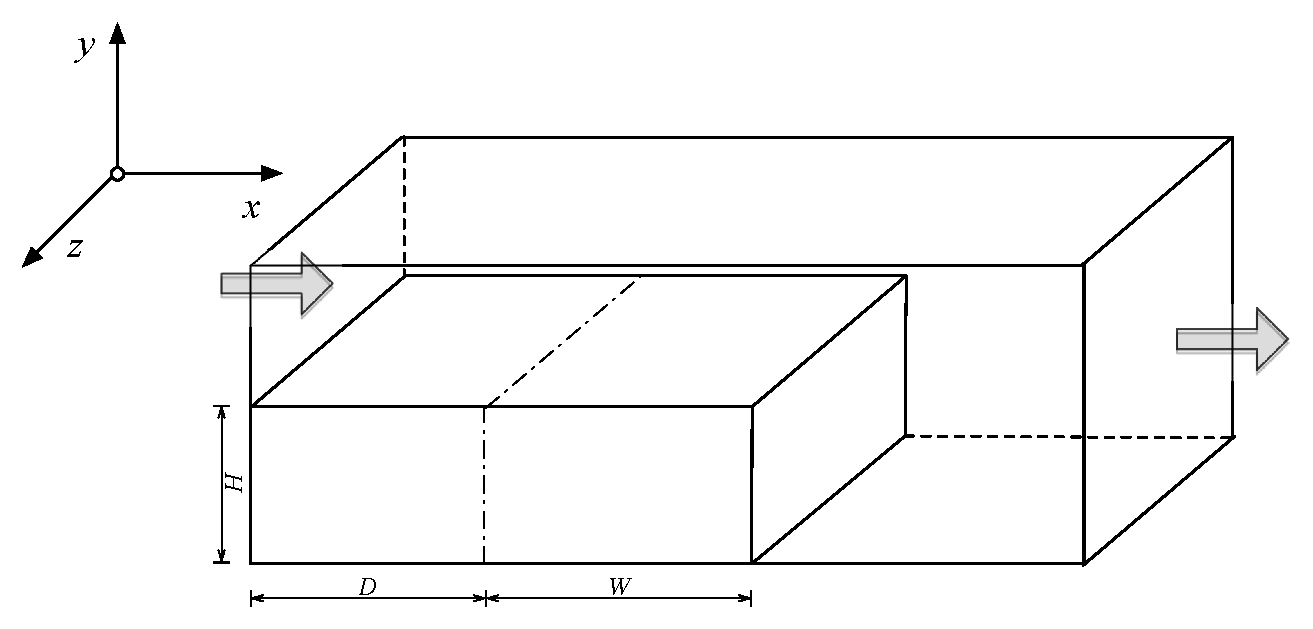
\includegraphics[width=14cm,clip]{Backstep.eps}
\end{center}
\caption{バックステップ流れの計算モデル.}
\label{fig:ip_backstep}
\end{figure}

\begin{table}[htdp]
\small
\caption{バックステップ問題のパラメータ.}
\begin{center}
\begin{tabular}{ll}\toprule
記号 & パラメータ\\ \midrule
Mode & 2D $|$ 3D\\ \hline
Width ($W$) & ステップの$x$方向の幅\\
Height ($H$) & ステップの$y$方向の高さ\\
Driver ($D$) & ドライバー部分の長さ($>0.0$でドライバあり,=0.0の場合ドライバーなし)\\
\bottomrule
\end{tabular}
\end{center}
\label{tbl:ip_backstep}
\end{table}

\begin{table}[htdp]
\small
\caption{バックステップ問題のID番号.}
\begin{center}
\begin{tabular}{ll}\toprule
ID & 属性\\ \midrule
1 & 流体\\
2 & 固体\\
3 & ドライバ部分の流体\\
4 & ドライバ流出面(流体)\\
\bottomrule
\end{tabular}
\end{center}
\label{tbl:ip_backstep_ID}
\end{table}

境界条件として,X-方向に流入,またはドライバ境界,X+方向は流出条件,Y-方向は壁面,Y+方向は壁面またはスリップ条件,Z$\pm$方向は壁面か周期境界を与えて計算します.二次元の問題を解く場合には,Mode=2Dを指定,VoxelSizeはkmax=3として,Z方向は周期境界条件を与えてください.

%
\subsection{IP\_CYLINDERクラス}
二次元と三次元の円柱・角柱まわりの流れを計算するクラスです.
\textbf{図\ref{fig:ip_cylinder}}と\textbf{表\ref{tbl:ip_cylinder}}に示すパラメータで計算空間を構成します.
断面形状は,円柱と角柱をShapeで指定します.それぞれの断面形状で指定するパラメータが異なります.
柱は$xy$平面の$z-$方向に接しています.これを基準に長さのパラメータを指定してください.

二次元の問題を解く場合には,Mode=2Dを指定,VoxelSizeはkmax=3としてください.この場合,パラメータ$W$は無視されます.

\begin{figure}[htdp]
\begin{center}
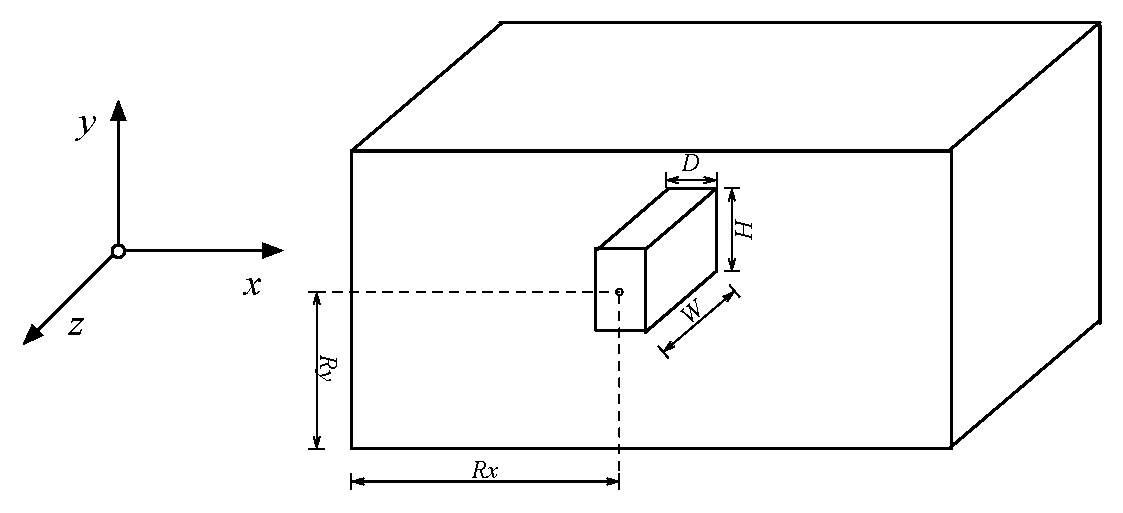
\includegraphics[width=14cm,clip]{Cylinder.eps}
\end{center}
\caption{円柱・角柱モデルの計算空間.}
\label{fig:ip_cylinder}
\end{figure}

\begin{table}[htdp]
\small
\caption{柱状物体の指定パラメータ}
\begin{center}
\begin{tabular}{ll}\toprule
記号 & パラメータ\\ \midrule
Mode & 2D $|$ 3D\\ 
Shape & Rectangular $|$ Circular\\ \hline
$D$ & 角柱を指定時の角柱の幅\\
$H$ & 角柱を指定時の角柱の高さ\\
$R$ & 円柱を指定時の半径\\
$W$ & 柱の$z$軸方向の長さ\\
$R_x$ & 柱の中心位置と$x$方向領域境界からの距離\\
$R_y$ & 柱の中心位置と$y$方向領域境界からの距離\\
\bottomrule
\end{tabular}
\end{center}
\label{tbl:ip_cylinder}
\end{table}

%
\subsection{IP\_Ductクラス}
\textbf{図\ref{fig:ip_duct}}のような円形と矩形のダクト流れを計算するモデルで,周期境界条件を用います.
流入面には,流れを発達させる機能をもつドライバー部分を指定することができます.

断面形状は,正方形または円形をShapeで指定し,
流入部の方向をDirectionで指定します.
ドライバー部は,Directionで指定した方向にドライバ部分が配置されます.
ドライバー部分を指定する場合には,Driverにその長さ$D$を指定してください.
$D=0.0$の場合には,ドライバー無しの指定になります.

\begin{figure}[htdp]
\begin{center}
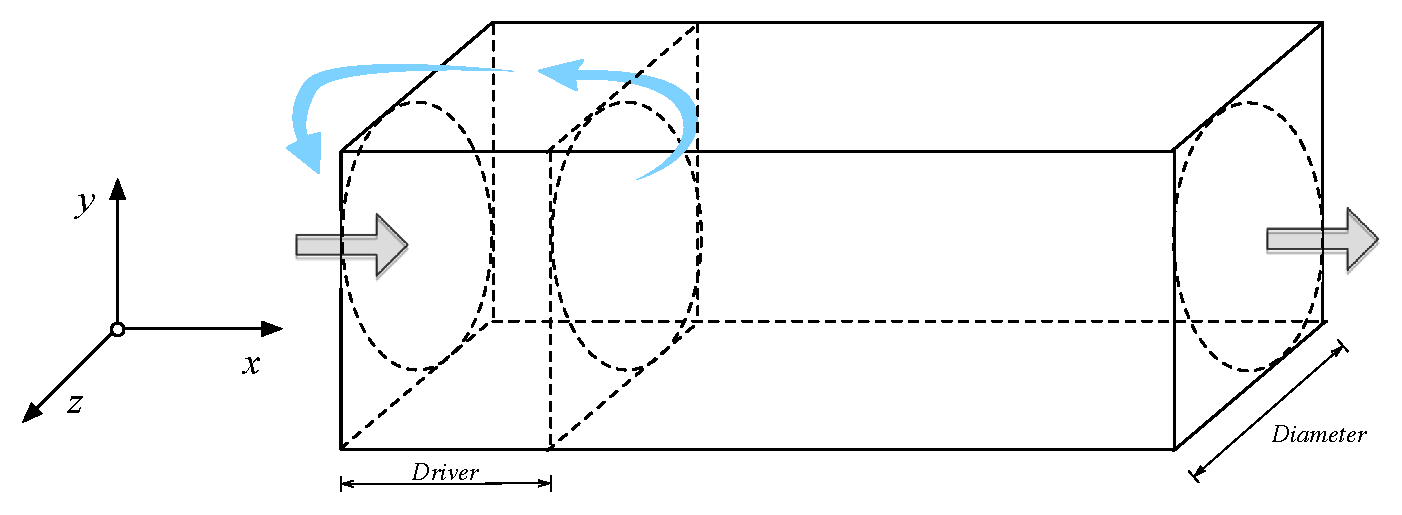
\includegraphics[width=16cm,clip]{Duct.eps}
\end{center}
\caption{ダクトの計算空間.$X-$方向にドライバ部を設置した場合.}
\label{fig:ip_duct}
\end{figure}

\begin{table}[htdp]
\small
\caption{ダクトの指定パラメータ}
\begin{center}
\begin{tabular}{ll}\toprule
記号 & パラメータ\\ \midrule
Shape & Rectangular $|$ Circular\\ \hline
Diameter & 正方形または円の直径\\
Direction & 周期境界と流入の方向(X\_minus, X\_plus, Y\_minus, Y\_plus, Z\_minus, Z\_plus)\\
Driver & ドライバー部分の長さ($>0.0$でドライバあり,=0.0の場合ドライバーなし)\\
\bottomrule
\end{tabular}
\end{center}
\label{tbl:ip_duct}
\end{table}


%
\subsection{IP\_PMTクラス}
CBCソルバークラスの基本的性能を測定するための例題クラスです.
三次元立方体の空間内のキャビティフローを解きます.
性能測定モードとなり,圧力反復の収束判定は行わず,反復回数は固定となります.
また,初期化時のファイル出力が抑制されます.

%
\subsection{IP\_PPLT2Dクラス}
二次元の平行平板間の流れを計算するためのクラスです.
\textbf{図\ref{fig:pplate2d}}のように辺長比が2:1の二次元空間を表現します.
z方向には3セルを設けており,単純な周期境界条件を用いて二次元を近似しています.
したがって,VoxelSizeでは\lq\lq kmax=3 \rq\rq を指定し,分割数imaxとjmaxの比は2:1となるように指定します.
空間格子幅は,x方向とy方向で同じ(直交等間隔)としています.

計算領域内部は単一媒質(セルID=1)が設定されています.
この例題は,パラメータ指定\lq\lq Unit\_of\_input\_parameter\rq\rq に無次元を指定します.

\begin{figure}[htdp]
\begin{center}
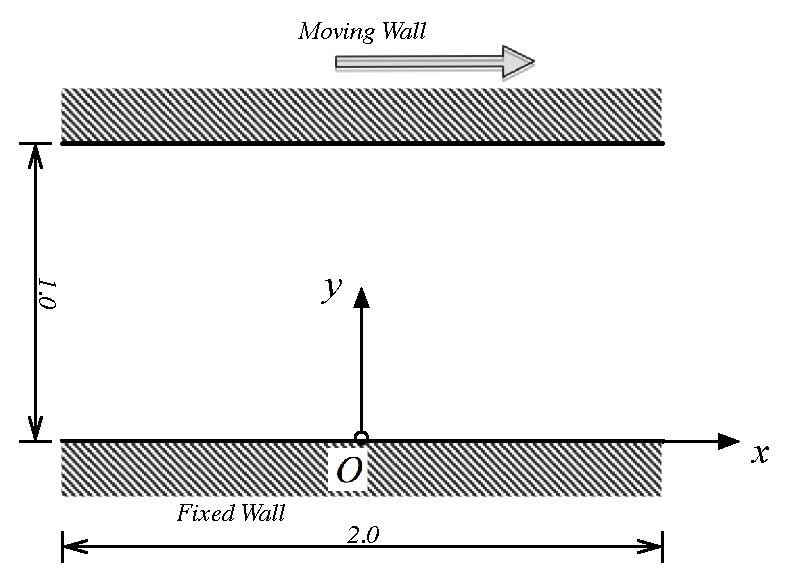
\includegraphics[width=8cm,clip]{PPLT2D.eps}
\end{center}
\caption{二次元平行平板間の計算空間.}
\label{fig:pplate2d}
\end{figure}


%
\subsection{IP\_Rectクラス}
IP\_Rectクラスは三次元の矩形の計算領域を表現するクラスで,計算領域内部は単一媒質(セルID=1)が設定されています.
計算領域は,次のようにDomainInfoタグで指定します.ここでは,各方向の分割数を64に指定し,基点座標が$(-0.5, -0.5, -0.5)$,ボクセルピッチを$pch=1.5625\times10^{-2}$に指定しています.
VoxelSizeとVoxelPitchのパラメータは,\textbf{図\ref{fig:rect intrinsic class}}に示すように,格子幅$pch$と分割数$imax$がそれぞれ対応しています.


{\small
\begin{program}
<DomainInfo>
  <VoxelOrigin ox="-0.5" oy="-0.5" oz="-0.5"/>
  <VoxelSize ix="64" jx="64" kx="64"/>
  <VoxelPitch dx="1.5625e-02" dy="1.5625e-02" dz="1.5625e-02"/>
</DomainInfo>
\end{program}
}


\begin{figure}[htdp]
\begin{center}
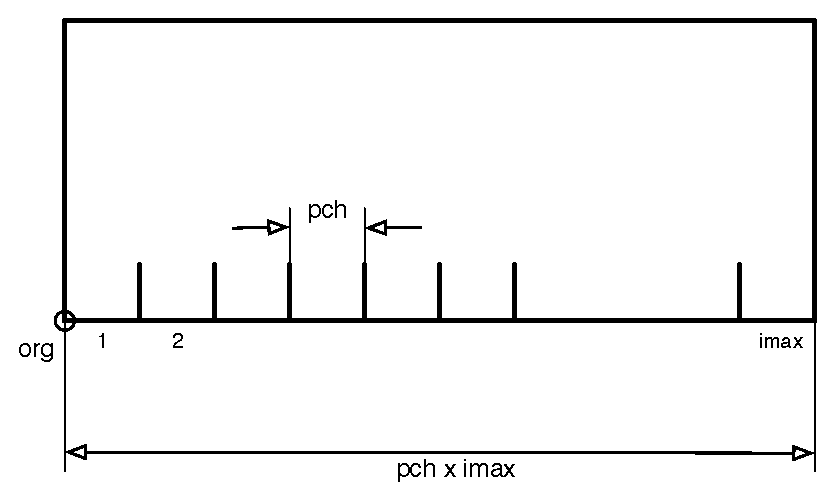
\includegraphics[width=9cm,clip]{rect.eps}
\caption{Rectangularクラスのパラメータ設定}
\label{fig:rect intrinsic class}
\end{center}
\end{figure}


\begin{table}[htdp]
\caption{Intrinsic\_Exampleタグで設定可能なパラメータ}
\begin{center}
\small
\begin{tabular}{lll}\toprule
指定パラメータ & 指定値 & 意味\\ \midrule
Check\_Even & Yes $|$ No & 分割数が偶数であるかどうかをチェックする\\
\bottomrule
\end{tabular}
\end{center}
\label{tbl:rect parameter}
\end{table}

\textbf{表\ref{tbl:rect parameter}}のパラメータは,Parameter $>$ Intrinsic\_Exampleセクションで指定します.

{ \small
\begin{program}
<Elem name="Intrinsic_Example">
  <Param dtype="STRING" name="Check_Even" value="Yes"/>
</Elem>
\end{program}
}

上記のパラメータ設定では,分割数の偶数チェックを行います.

%
\subsection{IP\_Polygonクラス}
XMLファイルで,\lq\lq Steer > Solver\_Property > Shape\_Approximation\rq\rq でDistance\_Infoを指定すると,距離情報を用いたスキームで計算します.
この\hypertarget{tgt:polygon_class}{IP\_Polygonクラス}は,入力するポリゴンファイルと,DomainInfoで指定する計算領域情報のみで計算を行うモデルテンプレートです.ポリゴンファイル名は,\lq\lq Steer > Polygon\_File\rq\rq で指定します.

%
\subsection{IP\_SHC1Dクラス}
\textbf{図\ref{fig:HC1D}}に示すような片持ちはりの熱伝導問題を一次元の定常熱伝導問題として解くためのクラスです.
この問題には厳密解があり,厳密解と計算結果を比較することにより予測精度の確認ができます.

\begin{figure}[htdp]
\begin{center}
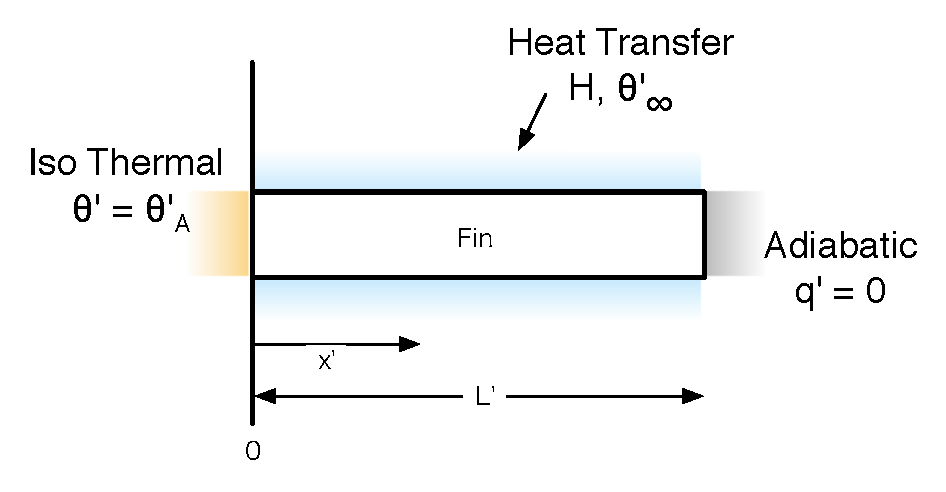
\includegraphics[width=9cm,clip]{1DHC.eps}
\end{center}
\caption{一次元定常熱伝導問題の模式図}
\label{fig:HC1D}
\end{figure}


計算領域は\textbf{図\ref{fig:HC model}}に示すようにx軸方向に放熱フィンをとり,y,z方向には5つだけセルを設けます.
領域の設定パラメータとして,x方向の分割数をimaxにより与えます.
放熱フィンを5分割したい場合には,imax=7を設定します.
その他の方向は$\mathrm{jmax=kmax=5}$で固定です.

例題と解析結果の詳細については,例題集をご覧ください.

\begin{figure}[htdp]
\begin{minipage}{0.47\hsize}
\begin{center}
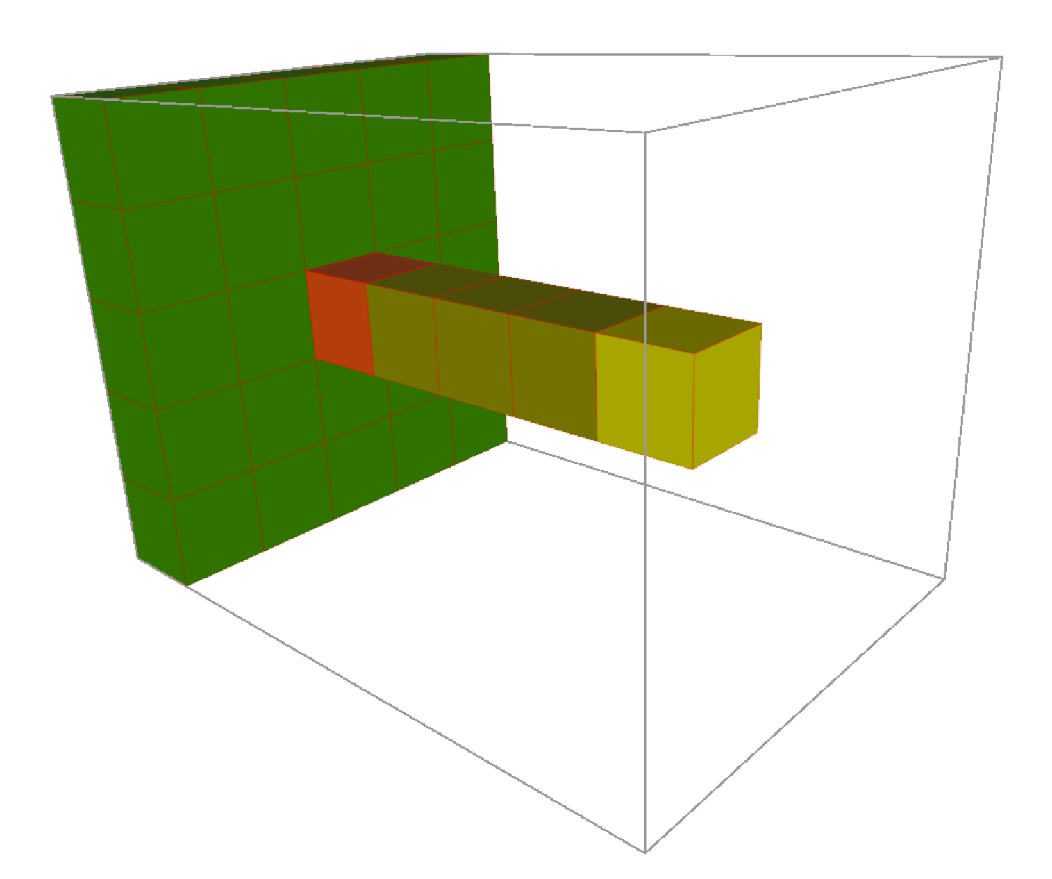
\includegraphics[height=5cm,clip]{model_iso.eps}
\end{center}
\end{minipage}
\begin{minipage}{0.47\hsize}
\begin{center}
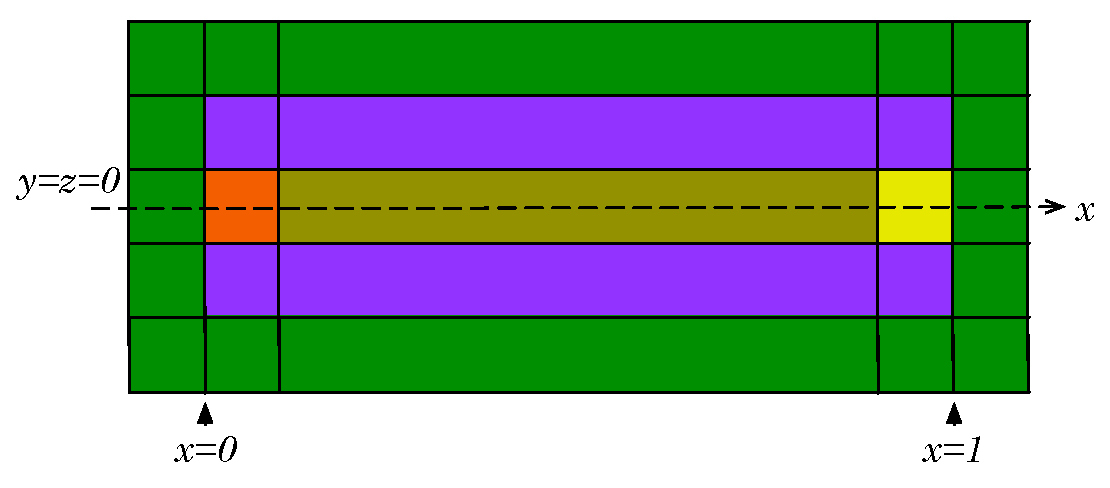
\includegraphics[height=3.5cm,clip]{dimension.eps}
\end{center}
\end{minipage}
\caption{一次元熱伝導問題を計算するための片持ち梁の三次元モデルとセルID (分割数が$7\times5\times5$の場合)}
\label{fig:HC model}
\end{figure}


\pagebreak
% 
\section{例題}
ソースファイルのExampleディレクトリに含まれる\hypertarget{tgt:samples}{例題}について説明します.
提供される例題は,組み込みモデルや簡単なボクセルモデルを同梱した例題群で,
基本的な流れやソルバーの検証のために用意されています.


\begin{table}[htdp]
\caption{組み込み例題}
\begin{center}
\small
\begin{tabular}{lll} \toprule
Example & Class & Comment\\ \midrule
Cavity flow 3D (Cube) & IP\_Rect & 三次元立方体キャビティフロー\\
LDC112  & IP\_Rect & Guermondの実験に対応する辺長が1:1:2のキャビティフロー\\ 
Duct 3D & IP\_Duct3D & ダクト流れ\\ 
PMT & IP\_PMT & 性能測定を行うための例題(三次元立方体キャビティフローの例題と同じ)\\
\bottomrule
\end{tabular}
\end{center}
\label{tbl:example at glance}
\end{table}

\begin{table}[htdp]
\caption{サンプル例題}
\begin{center}
\small
\begin{tabular}{lll} \toprule
Example & Comment\\ \midrule
Dragon & Asian Dragon周りの流れ\\
Heated Plate & 流体中の平板からの放熱\\
SHC1D & 熱伝導計算の解析解との比較\\ \bottomrule
\end{tabular}
\end{center}
\label{tbl:exercise}
\end{table}





%%%
\chapter{制御と物理パラメータ}
\label{chpt:param}
\begin{abstract}
V-Sphereシステム上の入力パラメータは,データベースなどでの再利用性を考慮し,XML(eXtensible Markup Language)形式で記述します.XMLはタグ構造のデータ記述言語で,階層的な要素の記述が可能なマークアップ言語です.このXMLデータをV-Sphere内部でツリー状のオブジェクトとして構文解析および操作します.
本章では,CBCソルバークラスの制御と物理パラメータ(これをコンフィギュレーションファイル\index{ふぁいる@ファイル!こんふぃぎゅれーしょん@コンフィギュレーション---}と呼びます)について説明します.境界条件の詳細については,CBCソルバークラス説明書をご覧ください.
\end{abstract}
%
\graphicspath{{./fig_Param/}}

%
\section{XMLコンフィギュレーションファイル}
%
\subsection{XML記述}
XML\index{XML}文書の先頭行は,\verb|<?xml version="1.0"?>|で始まり,このXML文書はXML 1.0 の規格を満たす文書であることを示しています.
XMLの要素は,\verb|<>..</>|で囲まれた対になったタグ\index{えっくすえむえる@XML!たぐ@---のタグ}で表現されます.ここでは,タグで囲まれている部分をセクション\index{えっくすえむえる@XML!せくしょん@---のセクション}と呼びます.
{
\small 
\begin{program}
<keyword>
	...
</keyword>
\end{program}
}


\noindent 一行内で終わるような短い要素の場合は,次のようにスラッシュで終わる形式で記述できます.
\vspace{2mm}

{
\small 
\begin{program}
<Param name="Output_Mode" dtype="STRING" value="forced" />
\end{program}
}

\noindent 要素を無効にする場合には,前後を\verb|<!-- *** -->|のように!と2連のマイナス記号で囲みます.
\vspace{2mm}

{
\small 
\begin{program}
<!--StartCondition type="Restart"/-->
\end{program}
}


%
\subsection{コンフィギュレーションファイルの構造}
コンフィギュレーションファイルは,ソルバークラスの入力ファイルとしての役割を果たします.
コンフィギュレーションファイルの中にあるSphereConfigタグ\index{SphereConfig}は,そこに記述された内容がV-Sphereのコンフィギュレーションであることを示します.クォーテーション(“”)で囲まれた文字列は,大文字でも小文字でもかまいません.

{
\small 
\begin{program}
<SphereConfig SolverType="CBC" >
	...
</SphereConfig>
\end{program}
}

\noindent \verb|SolverType="CBC"|\index{SolverType}は,V-Sphereが実行時にインスタンスするソルバクラスのキーワードを示します.このキーワードが,V-Sphereに登録されていない場合はエラーとなります.
SphereConfig内には,\textbf{表\ref{tbl:SphereConfig_tag}}に示すタグが記述されています.
コンフィギュレーションファイルの名称は任意で,このうち媒質情報と境界条件の内容の記述はSphereConfigタグ内に直接記述してもよいし,指定したファイルに記述しても構いません.両方存在する場合には,SphereConfigタグ内の記述が優先されます.\\

\begin{table}[htdp]
\caption{SphereConfig内のセクション}
\begin{center}
\small
\begin{tabular}{ll} \toprule
タグ & パラメータ\\ \midrule
DomainInfo & 計算領域\\
Steer & ソルバー制御\\
Parameter & 計算条件\\
BC\_Table & 境界条件\\
Medium\_Table & 媒質情報\\ \bottomrule
\end{tabular}
\end{center}
\label{tbl:SphereConfig_tag}
\end{table}


V-Sphereには,SPHERE定義要素\index{sphereていぎようそ@SPHERE定義要素}とソルバ定義要素\index{そるばていぎようそ@ソルバ定義要素}の2種類があります.SPHERE定義要素は,V-Sphereフレームワーク側で規定されたタグで,ソルバ定義要素はElem, Param要素で構成される汎用記述要素です.ソルバ定義要素のdtypeはデータの型(STRING, INT, REAL)を表し,valueは指定された型に対応した値をとります.

\pagebreak
%
\section{パラメータの詳細}
%
\subsection{DomainInfoセクション}
%
\subsubsection{DomainInfo}

\hypertarget{tgt:domaininfo}{DomainInfo}では,ボクセルモデル情報と外部ファイル情報を指定します.

\begin{indentation}{3zw}{0zw}

{\small
\begin{program}
<DomainInfo>
  <VoxelSize   ix="64" jx="64" kx="64" />
  <VoxelOrigin ox="0.0" oy="0.0" oz="0.0" />
  <VoxelPitch  dx="0.0" dy="0.0" dz="0.0" />
  <Param name="MDMTBL" dtype="STRING" value="xml/medium.xml" />
  <Param name="BCTBL"  dtype="STRING" value="xml/boundary.xml" />
  <Param name="MBXTBL" dtype="STRING" value="xml/multibox.xml">
</DomainInfo>
\end{program}
}

ボクセルモデル情報については,\textbf{表\ref{tbl:voxel info}}に示す計算領域に関するパラメータを指定します.この計算領域情報は,\hyperlink{tgt:example}{ユーザ問題と組み込み例題}とで指定内容が異なります.
組み込み例題の場合には,例題に応じて情報を指定します.
一方,ユーザ問題では,入力となる解析モデルファイルから,ボクセルのサイズやピッチなどのパラメータを取得します.

外部ファイル情報については,\textbf{表\ref{tbl:file info}}に示すように,媒質情報ファイル,境界条件情報ファイル,多連結領域の分割情報について,外部ファイルとして記述する場合にファイルのパスを指定できます.

\begin{table}[htdp]
\caption{DomainInfoセクションにおける計算領域パラメータの指定}
\begin{center}
\small
\begin{tabular}{ll} \toprule
タグ & 指定内容\\ \midrule
VoxelSize & 計算空間の各軸方向の分割数\\
VoxelOrigin & 計算空間における座標値の最小値\\
VoxelPitch & 各軸方向の分割幅\\
VoxelWidth & 計算領域の大きさ\\ \bottomrule
\end{tabular}
\end{center}
\label{tbl:voxel info}
\end{table}

\begin{table}[htdp]
\caption{外部ファイル指定}
\begin{center}
\small
\begin{tabular}{ll} \toprule
タグ & 説明\\ \midrule
MDMTBL & 媒質情報を記述したコンフィギュレーションファイルの指定\\
BCTBL  & 境界条件を記述したコンフィギュレーションファイルの指定\\
MBXTBL & 多連結領域分割計算時の分割情報ファイルの指定\\ \bottomrule
\end{tabular}
\end{center}
\label{tbl:file info}
\end{table}

\end{indentation}

\pagebreak
%
\subsection{Steerセクション}
\label{sec:steer}
Steerセクションでは,CBCソルバークラスの実行制御パラメータ\index{じっこうせいぎょぱらめーた@実行制御パラメータ}を記述します.\\

%
\subsubsection{Algorithm}

時間積分と\hypertarget{tgt:algorithm}{解法アルゴリズム}の組み合わせを選択するパラメータです.

\begin{indentation}{3zw}{0zw}

{\small
\begin{program}
<Elem name="Algorithm">
  <Param name="Flow"   dtype="STRING" value="FS_C_EE_D_EE"/>
  <Param name="Heat"   dtype="STRING" value="C_EE_D_EE"/>
</Elem>
\end{program}
}

\textbf{表\ref{tbl:alg_flow}}に時間進行法と分離解法の種類の組み合わせを示します.Flowパラメータでは流動の支配方程式の時間積分法と解法アルゴリズムの組み合わせを指定します.
%時間二次精度以上を選択した場合には,\verb|Convection_Term|\ref{sec:p_convection}では二次以上の空間スキームしか選択できません.\\

\begin{table}[htdp]
\caption{流動解析のアルゴリズム選択パラメータ指定}
\begin{center}
\small
\begin{tabular}{ll} \toprule
キーワード & 時間積分法と解法の組み合わせ\\ \midrule
FS\_C\_EE\_D\_EE & Fractional Step法 + 時間一次精度Euler陽解法(対流項と拡散項)\\ \bottomrule
%FS\_C\_RK\_D\_CN & FS法 + 時間二次精度 Runge-Kutta陽解法(対流項)+ Crank-Nicholson陰解法(拡散項)\\
%FS\_C\_RK\_D\_ME & FS法 + 時間二次精度 Runge-Kutta陽解法(対流項)+ Modified-Euler陽解法(拡散項)\\
%FS\_C\_AB\_D\_AB & FS法 + 時間二次精度 Adams-Bashforth陽解法(対流項と拡散項)\\ \bottomrule
\end{tabular}
\end{center}
\label{tbl:alg_flow}
\end{table}

温度解析の場合には,Heatパラメータで温度輸送方程式の時間進行法と解法アルゴリズムの組み合わせを示します.指定できるパラメータは\textbf{表\ref{tbl:alg_heat}}に示します.\\

\begin{table}[htdp]
\caption{温度解析のアルゴリズム選択パラメータ指定}
\begin{center}
\small
\begin{tabular}{ll} \toprule
キーワード & 時間積分法と解法の組み合わせ\\ \midrule
C\_EE\_D\_EE & 時間一次精度 Euler陽解法(対流項と拡散項)\\
C\_EE\_D\_EI & 時間一次精度 Euler陽解法(対流項)+ Euler陰解法(拡散項)\\ \bottomrule
%C\_AB\_D\_AB & 時間二次精度 Adams-Bashforth陽解法(対流項と拡散項)\\ \bottomrule
\end{tabular}
\end{center}
\label{tbl:alg_heat}
\end{table}
\end{indentation}



%%%
\pagebreak
\subsubsection{Average\_Option}

\hypertarget{tgt:average_option}{時間平均操作}に関するパラメータを指定します.

\begin{indentation}{3zw}{0zw}

{\small
\begin{program}
<Elem name="Average_Option">
  <Param name="Operation"    dtype="STRING" value="On" />
  <Param name="Start_Type"   dtype="string" value="time" />
  <Param name="Start"        dtype="REAL"   value="500.0" />
</Elem>
\end{program}
}

\textbf{表\ref{tbl:averaging}}に物理量の時間平均操作\index{じかんへいきんそうさ@時間平均操作}を指定するパラメータを示します.
CBCソルバークラスは非定常解析を行いますので,流れの挙動が準定常状態になったところで時間平均操作を開始し,十分な長さで時間平均操作が行われた速度場や温度場を定常解\index{ていじょうかい@定常解}とみなします.
時間平均操作の開始時刻はStartで指定し,この開始時刻以降,毎ステップごとに時間平均操作を行います.
平均操作の開始時刻は,Start\_Typeで指定する方法に依存し,
Timeを指定した場合にはUnit\_of\_Input\_Parameterの次元に従います.
つまり,\hyperlink{tgt:unit}{value}=\lq\lq DIMENSIONAL\rq\rq の場合には有次元時刻で時間平均操作の開始時刻を指定することになります.

時間平均場の出力タイミングは,\hyperlink{tgt:fileio}{File\_IO}のAveraged\_Intervalで指定します.


\begin{table}[htdp]
\caption{Average\_Optionのパラメータ}
\begin{center}
\small
\begin{tabular}{ll} \toprule
キーワード & 指定パラメータ\\ \midrule
Operation & On $|$ Off\\
Start\_Type & 開始時刻の指定 (Step $|$ Time)\\
Start & 時間平均操作の開始時刻\\ \bottomrule
\end{tabular}
\end{center}
\label{tbl:averaging}
\end{table}

\end{indentation}



%%%
\pagebreak
\subsubsection{Check\_Parameter}

ボクセルモデルと入力パラメータの\hypertarget{tgt:check_parameter}{整合性のチェック}を行い,初期設定後にソルバーを停止します.

\begin{indentation}{3zw}{0zw}

{\small
\begin{program}
<Param name="Check_Parameter" dtype="STRING" value="On"/>
\end{program}
}

Check\_Parameter=\lq\lq On\rq\rq でチェックが有効な場合,V-Sphereを起動してパラメータを読み込み,前処理が終了した段階でCBCソルバーを強制終了します.
このとき,初期設定パラメータの内容がconditions.txtに書き出されているので,パラメータのチェックができます.
また,初期条件を与えたフィールドファイルが出力されるので,初期条件のチェックが可能です.

\end{indentation}



%%%
\pagebreak
\subsubsection{Convection\_Term}

\hypertarget{tgt:convection_term}{対流項のスキーム}に関するパラメータを指定します.

\begin{indentation}{3zw}{0zw}

{\small
\begin{program}
<Elem name="Convection_Term">
  <Param name="Scheme"   dtype="STRING" value="O3_MUSCL" />
  <Param name="Limiter"  dtype="STRING" value="minmod" />
</Elem>
\end{program}
}

SchemeとLimiterのパラメータを\textbf{表\ref{tbl:scheme limiter}}に示します.Limiterは制限関数\index{せいげんかんすう@制限関数}の種類を示し,Schemeが\verb|O3_MUSCL|の場合のみ有効となります.
非圧縮流れのように物理量の変化が連続的な場合には不要の場合もあります.
ファイル出力時のオプションでガイドセル出力\hyperlink{tgt:fileio}{Guide\_Out}=\lq\lq with\rq\rq を指定している場合には,対流項スキームによってステンシル\index{ステンシル}が変化するので,ガイドセル\index{ガイドセル}の値も異なります.

\begin{table}[htdp]
\small
\caption{SchemeとLimiterのパラメータ}
\begin{minipage}{.6\textwidth}
\begin{center}
\begin{tabular}{llc} \toprule
Scheme & 指定スキーム & 出力ガイドセルサイズ\\ \midrule
O1\_Upwind & 一次精度風上スキーム & 1\\
O2\_Central & 二次精度中心スキーム & 1\\
O3\_MUSCL & 三次精度MUSCLスキーム & 2\\ \bottomrule
\end{tabular}
\end{center}
\end{minipage} \hfill
\begin{minipage}{.38\textwidth}
\begin{center}
\begin{tabular}{ll} \toprule
Limiter & 制限関数\\ \midrule
Minmod & minmod型\\
No\_Limiter & | \\ \bottomrule
\end{tabular}
\end{center}
\end{minipage}
\label{tbl:scheme limiter}
\end{table}

\end{indentation}



%%%
\pagebreak
\subsubsection{Derived\_Variable}

\hypertarget{tgt:derived_variable}{派生変数}(基本変数から計算される変数)の生成を指定します.

\begin{indentation}{3zw}{0zw}

{\small
\begin{program}
<Elem name="Derived_Variable">
  <Param name="Total_Pressure"       dtype="STRING" value="off" />
  <Param name="2nd_Invariant_of_VGT" dtype="STRING" value="on" />
  <Param name="Helicity"             dtype="STRING" value="on" />
  <Param name="Vorticity"            dtype="STRING" value="on" />
</Elem>
\end{program}
}

\textbf{表\ref{tbl:derived vars}}に示す各変数は,on/offのスイッチ指定により有効・無効になり,\hyperlink{tgt:fileio}{File\_IO}セクションのInstant\_Intervalで指定するタイミングでファイルに出力されます.value=\lq\lq off\rq\rq の場合には,OutFileタグの記述は無効となります.OutputDataセクションのIntervalでは設定しません.

\begin{table}[htdp]
\caption{派生変数の指定}
\begin{center}
\small
\begin{tabular}{ll}\toprule
タグ & 生成する派生変数\\ \midrule
Total\_Pressure & 全圧\\
Vorticity & 渦度ベクトル\\
Helicity & ヘリシティ\\
2nd\_Invariant\_of\_VGT & 速度勾配テンソルの第二不変量\\ \bottomrule
\end{tabular}
\end{center}
\label{tbl:derived vars}
\end{table}

%
\paragraph{全圧(総圧)}
全圧の計算を指定した場合には,同時に\hyperlink{tgt:output_data}{OutputData}セクションに出力ファイル名を次のように記述します.
attrタグにはTotalPressureを指定し,basenameには任意のプリフィックスを記述します\footnote{ここで指定するInterval属性は無効で,\hyperlink{tgt:interval}{Interval}セクションでの指定に従います.}.

{\small
\begin{program}
<OutFile attr="TotalPressure" Interval="1" format="SPH" basename="tp" />
\end{program}
}

全圧は次式で定義され,単位体積あたりのエネルギーを表します.

\begin{equation}
\frac{1}{2} {u^{\prime}}^{2} + \frac{P^{\prime}}{\rho^{\prime}} \qquad [Pa] \sim [J/m^3]
\label{eq:total pressure}
\end{equation}

非圧縮の場合には,

\begin{equation}
{P_{T}}^{\prime} \,=\, \frac{1}{2} \rho^{\prime} {u^{\prime}}^{2} + P^{\prime} \qquad [J/m^3]
\label{eq:total pressure icmp}
\end{equation}

\textbf{式(\ref{eq:total pressure icmp})}は無次元化すると,以下のようになります.

\begin{equation}
P_{T} \,=\, \frac{{P_{T}}^{\prime}}{\rho_{\mathit{0}}^{\prime} {u_{\mathit{0}}^{\prime}}^{2}}
\label{eq:total pressure icmp ND}
\end{equation}

%
\paragraph{渦度ベクトル}
渦度の計算を指定した場合には,同時に\hyperlink{tgt:output_data}{OutputData}セクションに出力ファイルを次のように記述します.
attrタグにはVorticityを指定し,basenameには任意のプリフィックスを記述します.

{\small
\begin{program}
<OutFile attr="Vorticity" Interval="1" format="SPH" basename="vrt" />
\end{program}
}

%
\paragraph{ヘリシティ}
ヘリシティは速度ベクトル$\overrightarrow{u}$と渦度ベクトル$\overrightarrow{\omega}$の内積として定義される量で次式により表せます.OutFileタグの記述は上記と同様です.

\begin{equation}
H \,=\, \overrightarrow{u} \cdot \overrightarrow{\omega}
\label{eq:helicity}
\end{equation}

{\small
\begin{program}
<OutFile attr="Helicity" Interval="1" format="SPH" basename="hlcty" />
\end{program}
}

%
\paragraph{速度勾配テンソルの第二不変量}
渦構造を可視化するのに利用され,
符号により単純剪断乱流の中の層状渦と管状渦を区別することができます\cite{tanaka:93:PF}.OutFileタグの記述は上記と同様です.
{\small
\begin{program}
<OutFile attr="2ndInvrntVGT" Interval="1" format="SPH" basename="i2vgt" />
\end{program}
}

\end{indentation}



%%%
\pagebreak
\subsubsection{Example}

\hypertarget{tgt:example}{解くべき問題}を指定します.

\begin{indentation}{3zw}{0zw}

{\small
\begin{program}
<Param name="Example" dtype="STRING" value="Users"/>
\end{program}
}

\textbf{表\ref{tbl:intrinsic_example}}にCBCソルバークラスで提供される組み込み例題\index{くみこみれいだい@組み込み例題}の一覧を示します.
表の中で,Usersはユーザーが準備した解析モデルを用いることを指定します.
組み込み例題で固有のパラメータ設定がある場合についてはParameter$\to$\hyperlink{tgt:intrinsic_example}{Intrinsic\_Example}をご覧ください.

また,具体的な例題の事例については,例題集をご覧ください.

\begin{table}[htdp]
\caption{Exampleのパラメータ指定}
\begin{center}
\small
\begin{tabular}{ll} \toprule
キーワード & 解く問題\\ \midrule
Cavity3D & 立方体キャビティ\\
Duct3D & 直方体と円形断面のダクト\\
LDC112 & 辺長比1:1:2の三次元キャビティ\\
Performance\_Test & 性能評価\\
SHC1D & 固体熱伝導\\
Users & ユーザの指定モデル\\ \bottomrule
\end{tabular}
\end{center}
\label{tbl:intrinsic_example}
\end{table}

\end{indentation}


%%%
\pagebreak
\subsubsection{File\_IO}

\hypertarget{tgt:fileio}{ファイル入出力モード}を指定します.このセクションでは,入出力ファイルの単位,ガイドセルのモード,ファイル出力モード,並列入出力モード,デバッグ時のファイルなどを指定します.

\begin{indentation}{3zw}{0zw}

{\small
\begin{program}
<Elem name="File_IO">
  <Param name="Unit_of_File"            dtype="STRING" value="non_Dimensional" />
  <Param name="Guide_Out"               dtype="STRING" value="with" />
  <Param name="Output_Mode"             dtype="STRING" value="Forced" />
  <Param name="Parallel_Input"          dtype="STRING" value="Master" />
  <Param name="Parallel_Output"         dtype="STRING" value="Master" />
  <Param name="Debug_divergence"        dtype="STRING" value="off" />
  <Param name="Instant_Interval_Type"   dtype="string" value="time" />
  <Param name="Instant_Interval"        dtype="real"   value="0.001" />
  <Param name="Averaged_Interval_Type"  dtype="string" value="step" />
  <Param name="Averaged_Interval"       dtype="real"   value="200" />
</Elem>
\end{program}
}

\textbf{表\ref{tbl:file_IO_parameter}}に指定するパラメータの内容を示します.
Unit\_of\_Fileでは入出力する結果ファイル(*.sph)の単位を指定し,有次元か無次元を指定できます.

Guide\_Outタグで\textbf{with}を指定した場合の出力ガイドセルのサイズは\hyperlink{tgt:convection_term}{Convection\_Term}の項を参照してください.


\begin{table}[htdp]
\caption{ファイル入出力のパラメータ指定}
\begin{center}
\small
\begin{tabular}{llll} \toprule
タグ & 指定項目 & キーワード & 指定内容 \\ \midrule
Unit\_of\_File & 入出力ファイルの単位 & Dimensional & 有次元\\
& & Non\_Dimensional & 無次元\\ \hline
Guide\_Out & ガイドセル出力モード & with & ガイドセルを一緒に出力\\
& & without & 内部領域のみ出力\\ \hline
Output\_Mode & ファイル出力モードの指定 & Every\_Time & 毎ステップ出力モード\\
& & Forced & 強制出力モード\\
& & Normal & 通常モード\\ \hline
Parallel\_Input & ファイル入力 & Master & マスターノードで単一ファイル入出力\\
& & Local  & ローカルノードで分散ファイル入出力 \\ \hline
Parallel\_Output & ファイル出力 & Master & マスターノードで単一ファイル入出力\\
& & Local  & ローカルノードで分散ファイル入出力 \\ \hline
Debug\_divergence & デバッグ時のファイル出力 & On$|$Off & $\nabla \cdot \bm{u}$の出力(無次元値)\\ \hline
Instant\_Interval\_Type & 瞬時値の出力指定形式 & Step & ステップ数指定\\
& & Time & 時間間隔の指定\\
Instant\_Interval & 出力間隔 & | & ステップ数$|$時間間隔\\ \hline
Averaged\_Interval\_Type & 平均値の出力指定形式 & Step & ステップ数指定\\
& & Time & 時間間隔の指定\\
Averaged\_Interval & 出力間隔 & | & ステップ数$|$時間間隔\\\bottomrule
\end{tabular}
\end{center}
\label{tbl:file_IO_parameter}
\end{table}

ファイル出力モードの指定は,3つのモードが指定できます.
\verb|Normal|の場合には,\hyperlink{tgt:interval}{Instant/Averaged\_Interval}で指定した出力間隔でファイルを出力します.
\verb|Forced|では,通常モードの動作に加えて\hyperlink{tgt:time_control}{Time\_Control}セクションのCalculation\_Periodで指定した終了時に必ずファイルを出力します.
また,\verb|Every_Time|を指定した場合には,毎ステップファイル出力を行います.

Parallel\_Input/Outputでは,並列計算時のファイル入出力のモードを指定します.
逐次実行の場合には,Masterを指定します.

デバッグのため,$\nabla \cdot \bm{u}$の値を無次元で出力します.ファイル名の指定は,\hyperlink{tgt:output_data}{OutputData}をご覧ください.

Intervalのキーワードにより,ファイル出力間隔を指定します.
対象となる出力ファイルに対して,時刻またはステップ数によりファイル出力間隔を指定できます.
Instant\_Interval\_TypeあるいはAveraged\_Interval\_Typeがvalue=\lq\lq time\rq\rq の場合,時刻の単位は\hyperlink{tgt:unit}{Unit\_of\_Input\_Parameter}で指定したモードに従います.
ファイルの指定については,\hyperlink{tgt:output_data}{OutputData}を参照してください.
\end{indentation}



%%%
\pagebreak
\subsubsection{InputData}

CBCソルバークラスで使用する\hypertarget{tgt:input_data}{入力ファイル情報}を指定します.

\begin{indentation}{3zw}{0zw}

{\small
\begin{program}
<InputData basedir=".">
  <InFile attr="SphereSVX"    format="svx" fname="example.svx" />
  <InFile attr="Pressure"     format="SPH" fname="prs0000000940.sph" />
  <InFile attr="Velocity"     format="SPH" fname="uvw0000000940.sph" />
  <InFile attr="AvrPressure"  format="SPH" fname="prsa0000000300.sph" />
  <InFile attr="AvrVelocity"  format="SPH" fname="uvwa0000000300.sph" />
</InputData>
\end{program}
}

InputDataセクションのbasedir要素で,ディレクトリを相対パスで指定する場合の起点を指定します.
\textbf{表\ref{tbl:infile}}にInFileタグで指定する入力ファイル\index{ふぁいる@ファイル!にゅうりょく@入力---}のパラメータを示します.
上記の例では,ボクセルファイルを指定する場合,attrに\lq\lq SphereSVX\rq\rq の属性情報を与え,フォーマットにsvxを指定しています.
ユーザ問題の場合には,ここで指定したファイル名を読み込み,計算を行います.attr属性に指定できるキーワードを\textbf{表\ref{tbl:infile_attr}}に示します.

ボクセルファイルのフォーマットにはsvxとsbxの2種類があります.svxフォーマットはセルID,体積率,面積率などを保持できるフォーマットですが,CBCソルバではセルIDのみを認識します.sbxフォーマットはセルIDと体積率を保持でき,zipにより圧縮されます.また,ファイルサイズを小さくするため,体積率は1Byte(255)で量子化されています.更に,1バイト内にセルID(6bit=64種類)と体積率(2bit,0,1とそれ以外の3状態)を記録するモードが利用できます.詳細はファイルフォーマットマニュアルをご覧ください.

リスタート\index{リスタート}を指定している場合には,このセクションでリスタートファイル名を指定する必要があります.

並列時のファイル入力のモードとして,マスターノードで全てのファイル入力を行うマスターモード,ローカルノードで担当計算領域のみを入力する分散モードがあります.
モードの指定は,\hyperlink{tgt:fileio}{File\_IO}を参照してください.

\begin{table}[htdp]
\caption{InputDataセクションのInFileのパラメータ指定}
\begin{center}
\small
\begin{tabular}{ll} \toprule
タグ & パラメータ\\ \midrule
attr & 属性情報\\
fname & 任意のファイル名\\
format & ファイルフォーマットの拡張子(svx $|$ sbx $|$ sph)\\ \bottomrule
\end{tabular}
\end{center}
\label{tbl:infile}
\end{table}

\begin{table}[htdp]
\caption{attr属性に指定可能なキーワード}
\begin{center}
\small
\begin{tabular}{ll} \toprule
キーワード & 指定内容\\ \midrule
SphereSVX & ボクセルファイル名(svxフォーマット)\\
SphereSBX & ボクセルファイル名(sbxフォーマット)\\
Pressure & 圧力のリスタートファイル名\\
Velocity & 速度のリスタートファイル名\\
Temperature & 温度のリスタートファイル名\\
AvrPressure & 時間平均圧力のリスタートファイル名\\
AvrVelocity & 時間平均速度のリスタートファイル名\\
AvrTemperature & 時間平均温度のリスタートファイル名\\ \bottomrule
\end{tabular}
\end{center}
\label{tbl:infile_attr}
\end{table}

\end{indentation}



%%%
\pagebreak
\subsubsection{Iteration}

圧力のポアソン方程式や陰解法のように,得られる線形システムの係数行列が大型疎行列となる場合には反復解法\index{はんぷくかいほう@反復解法}を用います.
ここでは流れと温度解析について,\hypertarget{tgt:iteration}{反復法のパラメータを指定}します.

\begin{indentation}{3zw}{0zw}

{\small
\begin{program}
<Elem name="Iteration">
  <Elem name="Flow">
    <Elem name="Poisson">
      <Param name="Iteration"     dtype="INT"    value="50"/>
      <Param name="Epsilon"       dtype="REAL"   value="1.0e-3"/>
      <Param name="Omega"         dtype="REAL"   value="1.2"/>
      <Param name="Norm"          dtype="STRING" value="v_div_max"/>
      <Param name="Linear_Solver" dtype="STRING" value="SOR2SMA" />
    </Elem>
  </Elem>
     
  <Elem name="Heat">
    <Elem name="Euler_Implicit">
      <Param name="Iteration"     dtype="INT"    value="30"/>
      <Param name="Epsilon"       dtype="REAL"   value="1.0e-2"/>
      <Param name="Omega"         dtype="REAL"   value="1.2"/>
      <Param name="Norm"          dtype="STRING" value="T_res_L2_absolute"/>
      <Param name="Linear_Solver" dtype="STRING" value="SOR" />
    </Elem>
  </Elem>
</Elem>
\end{program}
}

反復法を用いる場合は,\hyperlink{tgt:algorithm}{Algorithm}セクションで反復法を含む解法を指定します.
第2レベルで指定するElem\_nameのキーワードは,指定するアルゴリズムに応じて異なり,
\textbf{表\ref{tbl:itr_flow_algo}}に指定アルゴリズムと指定キーワードの関係を示します.
%2nd\_Poissonは二次精度Runge-Kutta法の場合の2nd stepの圧力反復の収束条件を意味します.

\textbf{表\ref{tbl:flow_itr}}には,流動解析の反復解法の指定パラメータを示します.
また,指定可能な収束判定ノルムの種類を\textbf{表\ref{tbl:norm-type}}に示します.


\textbf{表\ref{tbl:LS}}にCBCソルバークラスで選択できる反復解法を示します.
表中の△は,並列処理時のデータ依存性(再帰干渉)のために,逐次と並列時で異なる収束特性を示すことを意味します.
%SOR2CMAは反復過程でメモリアクセスが連続になるように並べ替えを行うためにオーバーヘッドが生じるので,反復回数が少ない場合には計算速度向上の効果はない.\\

\begin{table}[htdp]
\caption{流動解析のアルゴリズムと指定キーワード}
\begin{center}
\small
\begin{tabular}{ll} \toprule
Algorithm & 必要なキーワード\\ \midrule
FS\_C\_EE\_D\_EE & Poisson\\ \bottomrule
%FS\_C\_AB\_D\_AB & Poisson\\ \bottomrule
%FS\_C\_RK\_D\_ME & 1st\_Iteration, 2nd\_Iteration\\
%FS\_C\_RK\_D\_CN & 1st\_Iteration, 2nd\_Iteration\\ \bottomrule
\end{tabular}
\end{center}
\label{tbl:itr_flow_algo}
\end{table}

\begin{table}[htdp]
\caption{反復条件の指定}
\begin{center}
\small
\begin{tabular}{ll} \toprule
タグ & 指定内容\\ \midrule
Iteration & 最大反復回数\\
Epsilon & 収束閾値\\
Omega & 加速(緩和)係数\\
Norm & 収束ノルムの種類\\ 
Linear\_Solver & 反復法の指定\\ \bottomrule
\end{tabular}
\end{center}
\label{tbl:flow_itr}
\end{table}

\begin{table}[htdp]
\caption{流動計算における圧力反復のノルムの指定}
\begin{center}
\small
\begin{tabular}{lll} \toprule
キーワード & 収束判定基準 & 履歴出力のキーワード\\ \midrule
V\_Div\_Max & 発散の最大値 $max\left|div\,\bm{u}\right|$ & V\_Div\_Max\\
\vspace{2mm}
V\_Div\_Max\_Monitor & 発散の最大値 $max\left|div\,\bm{u}\right|$の値とセル位置を出力する\footnotemark[1] & V\_Div\_Max\\
\vspace{2mm}
V\_Div\_L2 & 発散の自乗和平方根 $\displaystyle \sqrt{ \sum_{i,j,k}^{Max}{{( {div\,\bm{u}} )}^2}}$ & V\_Div\_L2\\
\vspace{2mm}
P\_Res\_L2\_Absolute & 絶対残差のRMS $\displaystyle \sqrt{ \frac{1}{N} \sum_{i,j,k}^{Max} {\|\vec{b}- A \vec{x}\|}_{2} }$ & P\_Res\_L2\_A\\ 
P\_Res\_L2\_Relative & 相対残差のRMS $\displaystyle {\frac{ \sqrt{ \frac{1}{N} \sum_{i,j,k}^{Max}{\|\vec{b}- A \vec{x}\|}_{2}} } {\sum_{i,j,k}^{Max} {\|\vec{b}\|}_{2} }}$ & P\_Res\_L2\_R\\ \bottomrule
\end{tabular}
\end{center}
\label{tbl:norm-type}
\end{table}
\footnotetext[1]{サーチを行うので,実行速度は遅くなる(デバッグ利用).}

\begin{table}[htdp]
\caption{Linear\_Solverのパラメータ指定}
\begin{center}
\small
\begin{tabular}{llc} \toprule
キーワード & 反復解法 & 並列計算への適用\\ \midrule
Jacobi & 緩和Point Jacobi法 & ○\\
SOR & Point SOR法 & △\\
%SOR2CMA & 連続メモリアクセス型の2色SOR法\\
SOR2SMA & ストライドメモリアクセス型の2色SOR法 & ○\\ \bottomrule
\end{tabular}
\end{center}
\label{tbl:LS}
\end{table}

\pagebreak

温度計算で反復法を用いる場合は,\hyperlink{tgt:algorithm}{Algorithm}セクションで反復法を含む解法を指定します.

第2レベルで指定するElem\_nameのキーワードは,指定するアルゴリズムに応じて異なります.
\textbf{表\ref{tbl:itr_temp_algo}}に,指定アルゴリズムと指定キーワードの関係を示します.

温度解析の反復解法のパラメータは,\textbf{表\ref{tbl:flow_itr}}と同じです.
収束ノルムのタイプは\textbf{表\ref{tbl:norm-type4temp}}で指定します.

\begin{table}[htdp]
\caption{温度解析のアルゴリズムと指定キーワード}
\begin{center}
\small
\begin{tabular}{ll} \toprule
Algorithm &  必要なキーワード\\ \midrule
C\_EE\_D\_EE & | \\
%C\_AB\_D\_AB & なし\\
C\_EE\_D\_EI & Euler\_Implicit\\ \bottomrule
\end{tabular}
\end{center}
\label{tbl:itr_temp_algo}
\end{table}

\begin{table}[htdp]
\caption{温度計算における反復のノルムの指定}
\begin{center}
\small
\begin{tabular}{lll} \toprule
キーワード & 収束判定 & 履歴出力のラベル\\ \midrule
\vspace{2mm}
T\_Res\_L2\_Absolute & 絶対残差のRMS $\displaystyle \sqrt{ \frac{1}{N} \sum_{i,j,k}^{Max} {\|\vec{b}- A \vec{x}\|}_{2} }$ & T\_Res\_L2\_A\\ 
T\_Res\_L2\_Relative & 相対残差のRMS $\displaystyle {\frac{ \sqrt{ \frac{1}{N} \sum_{i,j,k}^{Max}{\|\vec{b}- A \vec{x}\|}_{2}} } {\sum_{i,j,k}^{Max} {\|\vec{b}\|}_{2} }}$ & T\_Res\_L2\_R\\ \bottomrule
\end{tabular}
\end{center}
\label{tbl:norm-type4temp}
\end{table}

\end{indentation}



%%%
\pagebreak
\subsubsection{LES\_Option}

\hypertarget{tgt:les_option}{LES}(Large-Eddy Simulation)のオプションパラメータを指定します\footnote{\today 現時点で機能未実装.}.

\begin{indentation}{3zw}{0zw}

{\small
\begin{program}
<Elem name="LES_Option">
  <Param name="LES_Calculation" dtype="STRING" value="on"/>
  <Param name="Model"           dtype="STRING" value="smagorinsky"/>
  <Param name="Cs"              dtype="REAL"   value="0.15"/>
  <Param name="Damping_factor"  dtype="REAL"   value="0.2"/>
</Elem>
\end{program}
}

指定できるLESのモデルを\textbf{表\ref{tbl:LES_model}}に示します.

\begin{table}[htdp]
\caption{LESのモデル指定}
\begin{center}
\small
\begin{tabular}{ll} \toprule
タグ & モデル\\ \midrule
Smagorinsky & 標準スマゴリンスキーモデル\\ \bottomrule
%Low\_Reynolds & 低レイノルズ数型モデル\\
%Dynamic & ダイナミックモデル\\ \bottomrule
\end{tabular}
\end{center}
\label{tbl:LES_model}
\end{table}

\end{indentation}



%%%
\pagebreak
\subsubsection{Log}

\hypertarget{tgt:log}{各種履歴}ファイル\index{ふぁいる@ファイル!りれき@履歴---}出力の制御パラメータを指定します.

\begin{indentation}{3zw}{0zw}

{\small
\begin{program}
<Elem name="Log">
  <Param name="Log_Base"              dtype="STRING" value="ON" />
  <Param name="Log_Iteration"         dtype="STRING" value="OFF" />
  <Param name="Log_Profiling"         dtype="STRING" value="ON" />
  <Param name="Log_Wall_Info"         dtype="STRING" value="Off" />
  <Param name="Console_Interval_Type" dtype="string" value="step" />
  <Param name="Console_Interval"      dtype="real"   value="1" />
  <Param name="History_Interval_Type" dtype="string" value="step" />
  <Param name="History_Interval"      dtype="real"   value="1" />
  <Param name="Unit_of_Log"           dtype="STRING" value="non_Dimensional" />
</Elem>
\end{program}
}

Log\_Baseタグでは,基本履歴ファイルのon/offを制御します.つまり,標準モニタ出力やコンポーネント情報,領域の流量収支履歴の出力を制御します.

Log\_Iterationタグは,各タイムステップの反復数,残差の最大値とそのインデクス値などの圧力の反復過程の履歴を出力します.
このタグを指定すると,残差は強制的に\hyperlink{tgt:iteration}{V\_Div\_Max}(発散の最大値)となり,\hyperlink{tgt:iteration}{Interation}タグでのノルムの指定は無効になります.反復履歴は他の種類のノルムには対応していません.

Log\_Profilingタグは,実行時に性能測定のための計時を行い,結果をレポートとして出力することを指定します.ログファイル名の指定は\hyperlink{tgt:output_data}{OutputData}セクションで行います.Detailオプションにより,詳細なレポートを出力します.出力項目の詳細は,\hyperlink{tgt:profile}{性能情報}をご覧ください.

Log\_Wall\_Infoは,\hyperlink{tgt:treatment_of_wall}{壁法則}を用いた場合の種々の情報を出力しますが,試験的なものです.

Intervalのキーワードにより,ファイル出力間隔を指定します.
対象となる出力ファイルに対して,時刻またはステップ数によりファイル出力間隔を指定できます.
Console\_Interval\_TypeあるいはHistory\_Interval\_Typeがvalue=\lq\lq time\rq\rq の場合,時刻の単位は\hyperlink{tgt:unit}{Unit\_of\_Input\_Parameter}で指定したモードに従います.
ログファイルのファイル名の指定は\hyperlink{tgt:output_data}{OutputData}セクションの\textbf{表\ref{tbl:logfile}}に示します.

Unit\_of\_Logではログ出力の有次元・無次元を指定します.

\begin{table}[htdp]
\caption{履歴ファイルの出力指定}
\begin{center}
\small
\begin{tabular}{lll} \toprule
タグ & 指定内容 & キーワード$|$指定内容\\ \midrule
Log\_Base & 標準履歴ファイル & ON $|$ OFF\\
Log\_Iteration & 反復解法の反復履歴 & ON $|$ OFF\\
Log\_Profiling & 実行性能レポートの作成・出力 & ON $|$ OFF\\
Log\_Wall\_Info & 壁面情報履歴 & ON $|$ OFF\\ \hline
Console\_Interval\_Type & 標準出力の出力指定形式 & Step (ステップ数指定)\\
& & Time (時刻指定)\\
Console\_Interval & 出力間隔 & ステップ数 $|$ 時刻\\ \hline
History\_Interval\_Type & 履歴ファイルの出力指定形式 & Step (ステップ数指定)\\
& & Time (時刻指定)\\
History\_Interval & 出力間隔 & ステップ数 $|$ 時刻\\ \hline
Unit\_of\_Log & ログファイル中の記述単位 & Dimensional $|$ Non\_Dimensional\\\bottomrule
\end{tabular}
\end{center}
\label{tbl:log_output}
\end{table}

\end{indentation}



%%%
\pagebreak
\subsubsection{Model\_Setting}

\hyperlink{tgt:medium_table}{Medium\_Table}セクションで記述する媒質ID\index{ばいしつあいでぃ@媒質ID}とボクセルモデル内のセルID\index{せるあいでぃ@ボクセルID}の\hypertarget{tgt:model_setting}{関係を記述}します.

\begin{indentation}{3zw}{0zw}

{\small
\begin{program}
<Elem name="Model_Setting">
  <Param name="fluid" id="1"    dtype="INT" value="800"  comment="air"/>
  <Param name="solid" id="310"  dtype="INT" value="600"  comment="wall"/>
</Elem>
\end{program}
}

上記の例では,セルID=1で指定される流体の物性値はMedium\_Tableにリストアップされる媒質ID=800であることを指定しています.同様に,セルID=310のボクセルは媒質ID=600により,その物性値が指定されます.
モデル作成時には,セルID $\ge$ 1である点に注意します.

\begin{table}[htdp]
\caption{セルIDと媒質IDの関連づけ}
\begin{center}
\small
\begin{tabular}{ll} \toprule
タグ & 説明\\ \midrule
Param name & セルの媒質の状態,Fluid or Solid\\
ID & セルID\\
value & 媒質ID\\
comment & コメント\\ \bottomrule
\end{tabular}
\end{center}
\label{tbl:model_tag}
\end{table}

\end{indentation}



%%%
\pagebreak
\subsubsection{Monitor\_List}

ユーザが指定した物理量を指定した位置で\hypertarget{tgt:monitor_list}{サンプリング}し,ファイルに出力する機能です.
サンプリングして出力する機能は2通りの方法で実装されています.
ここでは,指定した座標点で計算結果をサンプリングし,ファイルに出力する方法について説明します.
詳細は,第\ref{chpt:monitor}章をご覧ください.
もう一つの指定方法は,ボクセルモデルのセルIDを用いて指定する方法で,これについては\hyperlink{tgt:innerboundary}{境界条件}セクションをご覧ください.

\begin{indentation}{3zw}{0zw}

{\small
\begin{program}
<Elem name="Monitor_List"> 
  <Param name="Log"                    dtype="STRING" value="On" />
  <Param name="Output_File"            dtype="STRING" value="sample.log"/>
  <Param name="Output_Mode"            dtype="string" value="gather" />
  <Param name="Unit"                   dtype="STRING" value="non_Dimensional" />
  <Param name="Sampling_Interval_Type" dtype="string" value="step" />
  <Param name="Sampling_Interval"      dtype="real"   value="1" />

  <Elem name="point_set" comment="p1"> 
    <Param name="variable"        dtype="string" value="velocity" /> 
    <Param name="variable"        dtype="string" value="temperature" /> 
    <Param name="sampling_method" dtype="string" value="interpolation" /> 
    <Param name="sampling_mode"   dtype="string" value="all" /> 
    <Elem name="set" comment="10_Eng_ctr">
      <Param name="x" dtype="REAL" value="-0.217" /> 
      <Param name="y" dtype="REAL" value="-0.006" /> 
      <Param name="z" dtype="REAL" value="0.715" /> 
    </Elem> 
    <Elem name="set" comment="102_Eng_mnt_Rh_Fr"> 
      <Param name="x" dtype="REAL" value="-0.204" /> 
      <Param name="y" dtype="REAL" value="0.495" /> 
      <Param name="z" dtype="REAL" value="0.574" /> 
    </Elem> 
  </Elem> 

  <Elem name="line" comment="line_y=0"> 
    <Param name="variable"        dtype="string" value="velocity" /> 
    <Param name="division"        dtype="int"    value="64" /> 
    <Param name="sampling_method" dtype="string" value="smoothing" /> 
    <Param name="sampling_mode"   dtype="string" value="fluid" /> 
    <Elem name="from"> 
      <Param name="x" dtype="REAL" value="0.0" /> 
      <Param name="y" dtype="REAL" value="0.0" /> 
      <Param name="z" dtype="REAL" value="-0.5" /> 
    </Elem> 
    <Elem name="to"> 
      <Param name="x" dtype="REAL" value="0.0" /> 
      <Param name="y" dtype="REAL" value="0.0" /> 
      <Param name="z" dtype="REAL" value="0.5" /> 
    </Elem> 
  </Elem> 
</Elem> 
\end{program}
}

指定パラメータを\textbf{表\ref{tbl:monitor list}}に示します.
Monitor\_Listには,点群(point\_set)と線分(line)の2種類の指定方法があります.
それぞれをグループと呼び,point\_setの構成点をsetと定義します.

\begin{table}[htdp]
\caption{モニタリストでの指定パラメータ}
\begin{center}
\small
\begin{tabular}{lll} \toprule
タグ & 指定キーワード & 指定内容\\ \midrule
Log & On $|$ Off & ログ出力指定\\
Output\_File & | & 出力ファイル名\\
Output\_Mode & Gather & マスタープロセスに集約して出力\\
& Distribute & 各プロセス毎に出力\\
Unit & 入力パラメータと出力単位の指定 & Dimensional $|$ Non\_Dimensional\\
Sampling\_Interval\_Type & Step $|$ Time & 出力形式の指定\\
Sampling\_Interval & | & 指定間隔\\ \hline
Point\_Set & & 点群によりモニタ点を指定する\\
Set & & 点の座標を指定する\\
x,y,z & & 座標\\ \hline
Line & & 線分によりモニタ点を指定する\\
From & & 開始点を指定する\\
To & & 終了点を指定する\\
x,y,z & & 座標\\ \hline
Variable & Velocity & 速度を指定\\
 & Pressure & 圧力\\
 & Temperature & 温度\\
 & Total\_Pressure & 全圧\\
 & Vorticity & 渦度\\ \hline
%Velocity\_average & 速度の平均値\\
%Pressure\_average & 圧力の平均値\\
%Temperature\_average & 温度の平均値\\
%Total\_Pressure\_average & 全圧の平均値\\
Sampling\_Method & Nearest & モニタ指定点を含むセルの値\\
 & Interpolation & 三重線形内挿補間\\
 & Smoothing & 局所平均による平滑化\\ \hline
Sampling\_Mode & All & 全セルを対象とする\\
 & Fluid & 流体セルのみを対象とする\\
 & Solid & 固体セルのみを対象とする\\ \bottomrule
\end{tabular}
\end{center}
\label{tbl:monitor list}
\end{table}

\begin{itemize}
\item モニタ出力機能は,LogタグでON/OFFを指定します.
\item 出力ファイル名は,Output\_Fileタグで指定します.
\item 出力モードはOutput\_Modeタグで指定します.
これは並列計算時のファイル出力方式で,マスターノードに集約してファイル出力する場合にはGatherを指定し,分散ノード毎にファイル出力する場合にはDistributeを指定します.
\item Variableタグでは,サンプリングする物理量を指定します.
物理量はpoint\_setの例のように複数指定可能です.
\item Sampling\_Methodタグで指定されるパラメータは,サンプリング方法を指定します.
\item Sampling\_Modeで指定されるパラメータは,サンプリングモードを指定します.
\item ファイル出力間隔は,Sampling\_Intervalで指定し,その指定単位をSampling\_Interval\_Typeで指定します.
\item Unitタグでは,Monitor\_Listセクションで指定するパラメータの単位と出力するログの単位を指定します.指定パラメータと出力ログの単位は同じになります.
\end{itemize}

モニタリング指定された点はセルID=255が割り当てられ,測定位置情報が書き込まれたsvx/sbxファイルが出力されます.
\end{indentation}



%%%
\pagebreak
\subsubsection{OutputData}

\hypertarget{tgt:output_data}{出力}ファイル\index{しゅつりょくふぁいる@出力ファイル}の指定を行います.

\begin{indentation}{3zw}{0zw}

{\small
\begin{program}
<OutputData basedir=".">
  <History attr="log_base"       interval="1" fname="history_base.log" />
  <History attr="log_compo"      interval="1" fname="history_compo.log" />
  <History attr="log_domainflux" interval="1" fname="history_dommainflux.log" />
  <History attr="log_iteration"  interval="1" fname="history_iteration.log" />
  <History attr="log_wall_info"  interval="1" fname="history_wallinfo.log" />
  <OutFile attr="condition"      interval="1" format="ascii" basename="condition" />
  <OutFile attr="profiling"      interval="1" format="ascii" basename="profiling" />
  <OutFile attr="Velocity"       interval="1" format="SPH"   basename="vel"/>
  <OutFile attr="Pressure"       interval="1" format="SPH"   basename="prs"/>
  <OutFile attr="Temperature"    interval="1" format="SPH"   basename="tmp"/>
  <OutFile attr="AvrVelocity"    interval="1" format="SPH"   basename="vela"/>
  <OutFile attr="AvrPressure"    interval="1" format="SPH"   basename="prsa"/>
  <OutFile attr="AvrTemperature" interval="1" format="SPH"   basename="tmpa"/>
  <OutFile attr="Divergence"     interval="1" format="SPH"   basename="div" />
</OutputData>
\end{program}
}

\begin{itemize}
\item basedir要素では,指定ディレクトリを相対パスで指定する場合の起点を指定できます.
\item \textbf{表\ref{tbl:outfile}}にHistory, OutFileタグで指定するパラメータを示します.
\item basenameは出力するファイル名のプレフィックスを記述します.
ファイル名にはプレフィックスの後にタイムスタンプを表す数字が続き,拡張子がつきます.
\item ファイルフォーマットには,ascii, sph, fdvなどが指定できます.
\item 出力間隔はこのIntervalタグでは行わず,\hyperlink{tgt:interval}{Interval}セクションで指定します.
\item コンディションファイル(condition.txt)は,前処理計算が終了した時点で計算に関する設定や条件などが出力されます.
\item プロファイリングファイル(profiling.txt)は,実行性能の測定(実行時プロファイリング)情報が出力されます.
実行時プロファイリングの有効化の指定は,Logセクションの\hyperlink{tgt:log}{Log\_Profiling}で行います.
\end{itemize}


\begin{table}[htdp]
\caption{OutputDataセクションのパラメータ指定}
\begin{center}
\small
\begin{tabular}{ll} \toprule
タグ & 指定パラメータ\\ \midrule
attr & 属性情報(固定キーワード)\\
basename & 出力ファイルの接頭子\\
fname & 任意のファイル名\\
format & ファイルフォーマットの拡張子\\
interval & 出力ステップ間隔\\ \bottomrule
\end{tabular}
\end{center}
\label{tbl:outfile}
\end{table}

\pagebreak
履歴ファイルは\textbf{表\ref{tbl:logfile}}に示すものが指定できます.
Historyで指定される履歴ファイルの出力インターバルはLogセクションの\hyperlink{tgt:log}{History\_Interval}で指定します.
XMLによるサンプリングについては\hyperlink{tgt:monitor_list}{Monitor\_List}を参照してください.

並列時のファイル出力のモードとして,マスターノードで全てのファイル出力を行うマスターモード,ローカルノードで担当計算領域のみを入出力する分散モードがあります.
モードの指定はFile\_IOセクションの\hyperlink{tgt:fileio}{Parallel\_Output}を参照してください.

\begin{table}[htdp]
\caption{履歴ファイルおよび結果出力ファイルの種類}
\begin{center}
\small
\begin{tabular}{ll} \toprule
attr & 履歴の種類\\ \midrule
log\_base & 標準履歴ファイル(モニタ出力)\\
log\_compo & コンポーネントに関する履歴\\
log\_domainflux & 計算領域の外部境界における流束の履歴\\
log\_iteration & 反復履歴\\ 
log\_wall\_info & 壁面情報\\
Pressure & 圧力の瞬間値\\
Velocity & 速度の瞬間値\\
Temperature & 温度の瞬間値\\
AvrPressure & 圧力の平均値\\
AvrVelocity & 速度の平均値\\
AvrTemperature & 温度の平均値\\
TotalPressure & 反復履歴\\ 
Vorticity & XML指定のサンプリング履歴\\
Helicity & 壁面情報\\ 
2ndInvrntVGT & 速度勾配テンソルの第二不変量\\ 
Divergence & 速度の発散値(無次元)\\ \bottomrule
\end{tabular}
\end{center}
\label{tbl:logfile}
\end{table}

\end{indentation}

%%%
\pagebreak
\subsubsection{Polygon\_File}
\hypertarget{tgt:poly_file_name}{ポリゴンファイル名}を指定します.

\begin{indentation}{3zw}{0zw}
\small

\hyperlink{tgt:solver_property}{Shape\_Approximation}でDistance\_Infoを指定すると,距離情報を用いたスキームでの計算となります.この場合,ポリゴンファイルが必要となりますが,そのポリゴンファイルを記述したファイル名をこのセクションで指定します.
ポリゴンファイルと\hyperlink{tgt:domaininfo}{DomainInfo}の指定のみで計算をする場合には,\hyperlink{tgt:polygon_class}{IP\_Polygonクラス}を指定します.

\begin{program}
<Elem name="Polygon_File">
  <Param name="File_Name" dtype="string" value="polygon.xml"/>
</Elem>
\end{program}

\end{indentation}

%%%
\pagebreak
\subsubsection{Reference\_Frame}

\hypertarget{tgt:reference_frame}{観測}の座標系\index{ざひょうけい@座標系}を指定します.

\begin{indentation}{3zw}{0zw}
\small

\begin{program}
<Elem name="Reference_Frame">
  <Param name="Reference_Frame_Type" dtype="string" value="translation"/>
  <Param name="u" dtype="REAL" value="0.0"/>
  <Param name="v" dtype="REAL" value="0.0"/>
  <Param name="w" dtype="REAL" value="0.0"/>
</Elem>
\end{program}

\normalsize
CBCソルバークラスでは,\textbf{表\ref{tbl:ref_frame}}に示す選択肢があります.
移動座標系\index{ざひょうけい@座標系!いどう@移動---}を指定する場合には,格子の移動速度の各方向成分(有次元では$[m/s]$)を入力します.
座標系は右手系をとり,各軸x, y, z方向の速度成分をそれぞれu, v, wとします.
静止座標系\index{ざひょうけい@座標系!せいし@静止---}と移動座標系とでは,同じ問題を解く場合でも与える境界条件が異なるので注意します.

\begin{table}[htdp]
\caption{Reference\_Frameの指定}
\begin{center}
\small
\begin{tabular}{lll} \toprule
タグ & 指定パラメータ & 参照座標系\\ \midrule
Stationary & | & 静止座標系\\
Translational & $u,\,v,\,w$ & 並進運動する移動座標系\\ \bottomrule
%Rotational & $u,\,v,\,w$ & 回転運動する座標系\\ \bottomrule
\end{tabular}
\end{center}
\label{tbl:ref_frame}
\end{table}

\end{indentation}



%%%
\pagebreak
\subsubsection{StartCondition}

計算の\hypertarget{tgt:start_condition}{スタート方法}を指定します.

\begin{indentation}{3zw}{0zw}

{\small
\begin{program}
<StartCondition type="Initial"/>
\end{program}
}

\textbf{表\ref{tbl:start}}に選択肢を示します.リスタート\index{リスタート}の場合,ファイルは\hyperlink{tgt:input_data}{InputData}セクションのInFileで指定します.

\begin{table}[htdp]
\caption{Start Conditionのパラメータ指定}
\begin{center}
\small
\begin{tabular}{ll} \toprule
タグ & スタートの種類\\ \midrule
Initial & ゼロスタート\\
Restart & リスタート\\ \bottomrule
\end{tabular}
\end{center}
\label{tbl:start}
\end{table}

\end{indentation}



%%%
\pagebreak
\subsubsection{Solver\_Property}

CBCソルバーの\hypertarget{tgt:solver_property}{基本的なパラメータ}を設定します.ここでは,支配方程式の型の選択,浮力モード,形状近似などのパラメータを指定します.

\begin{indentation}{3zw}{0zw}

{\small
\begin{program}
<Elem name="Solver_Property">
  <Param name="Basic_Equation"       dtype="STRING" value="Incompressible"/>
  <Param name="Buoyancy"             dtype="STRING" value="No_Buoyancy" />
  <Param name="Kind_of_Solver"       dtype="STRING" value="Flow_Only" />
  <Param name="PDE_type"             dtype="STRING" value="Navier_Stokes" />
  <Param name="Shape_Approximation"  dtype="STRING" value="binary" />
  <Param name="Time_Variation"       dtype="STRING" value="Unsteady" />
</Elem>
\end{program}
}

Basic\_Equationには,\textbf{表\ref{tbl:basic_eq}}に示す支配方程式の形式を示します.

\begin{table}[htdp]
\caption{Basic\_Equationのパラメータ指定}
\begin{center}
\small
\begin{tabular}{ll} \toprule
タグ & 支配方程式\\ \midrule
%Compressible & 圧縮性\\ \bottomrule
Incompressible & 非圧縮性\\ \bottomrule
%Limited\_Compressibility & 微小圧縮性\\ \bottomrule
\end{tabular}
\end{center}
\label{tbl:basic_eq}
\end{table}

PDE\_typeで指定する方程式の型は,\textbf{表\ref{tbl:PDE type}}から選択します.
デフォルトでNavier Stokesで,Eulerはテスト用のパラメータです.

\begin{table}[htdp]
\caption{PDE\_typeのパラメータ指定}
\begin{center}
\small
\begin{tabular}{ll} \toprule
タグ & PDEの型\\ \midrule
Navier-Stokes & Navier-Stokes方程式\\
Euler & Euler方程式\\ \bottomrule
\end{tabular}
\end{center}
\label{tbl:PDE type}
\end{table}

Kind\_of\_Solverには,\textbf{表\ref{tbl:kos}}に計算する問題の熱流動現象の分類(熱流動タイプ\index{ねつりゅうどうたいぷ@熱流動タイプ})を示します.
熱伝導方程式を指定している場合(Kind\_Of\_Solver=\lq\lq SOLID\_CONDUCTION\rq\rq )には,Heat Conduction Equationと表示されます.
また,Buoyancyの指定は,Kind\_of\_Solverが必要とする場合にのみ有効になります.

\begin{table}[htdp]
\caption{熱対流計算とKind\_Of\_SolverおよびBuoyancyの関係}
\begin{center}
\small
\begin{tabular}{lll} \toprule
支配方程式 & Kind\_of\_Solver & Buoyancy\\ \midrule
純強制対流 & Flow\_Only & |\\
強制熱対流(浮力なし)& Thermal\_Flow & No\_Buoyancy\\
強制熱対流(浮力あり)& Thermal\_Flow & Boussinesq\\
%& & Low\_Mach\\
自然対流 & Thermal\_Flow\_Natural & Boussinesq\\
%& & Low\_Mach\\
固体熱伝導 & Solid\_Conduction & |\\ \bottomrule
%共役熱移動 & Conjugate\_Heat\_Transfer & Boussinesq\\ 
%& & Low\_Mach\\ \bottomrule
\end{tabular}
\end{center}
\label{tbl:kos}
\end{table}

\pagebreak
Shape\_Approximationタグには,\textbf{表\ref{tbl:ShapeApprox}}に示す解析モデルの形状近似モードを指定します.

\begin{table}[htdp]
\caption{形状近似モードの指定}
\begin{center}
\small
\begin{tabular}{ll} \toprule
タグ & 形状近似\\ \midrule
Binary & バイナリボクセル近似\\  \bottomrule
Distance\_Info & 距離情報近似\\
%Implicit\_Function & 陰関数近似\\ 
%Level\_Set & レベルセット関数近似\\
%Volume\_Fraction & 体積率近似\\ \bottomrule
\end{tabular}
\end{center}
\label{tbl:ShapeApprox}
\end{table}

Time\_Variationタグでは,\textbf{表\ref{tbl:steady}}に示すパラメータにより,解析する現象として定常あるいは非定常を指定します.
\begin{table}[htdp]
\caption{非定常モードの指定}
\begin{center}
\small
\begin{tabular}{ll} \toprule
タグ & モードの指定\\ \midrule
Steady & 定常\\
Unsteady & 非定常\\ \bottomrule
\end{tabular}
\end{center}
\label{tbl:steady}
\end{table}

\end{indentation}



%%%
\pagebreak
\subsubsection{Time\_Control}

\hypertarget{tgt:time_control}{時刻設定}に関するパラメータを指定します.

\begin{indentation}{3zw}{0zw}

{\small
\begin{program}
<Elem name="Time_Control">
  <Param name="Acceleration_Type"  dtype="string" value="time" />
  <Param name="Acceleration"       dtype="REAL"   value="0.0" />
  <Param name="Dt_Type"            dtype="string" value="CFL_Reference_Velocity" />
  <Param name="Delta_t"            dtype="REAL"   value="0.1" />
  <Param name="Period_Type"        dtype="string" value="time" />
  <Param name="Calculation_Period" dtype="REAL"   value="5.0" />
</Elem>
\end{program}
}

%
\paragraph{Acceleration}
Accelerationタグは,イニシャルスタート\index{イニシャルスタート}の場合にのみ有効なパラメータで,一定速度になるまでの時間を指定します.
Acceleration\_Typeで指定する時間の単位を指定します.
指定単位がTimeの場合,加速時間の値はUnitセクションの\hyperlink{tgt:unit}{Unit\_of\_Input\_Parameter}で指定するモード(Dimensional/Non\_Dimensional)に従います.計算初期の急加速による発散を防ぐため,格子の移動速度や指定流速をゼロから徐々に加速し,指定の値に漸近させる目的で利用します.
加速時間を長くとると流れの発達に時間がかかるので,発散しない程度の時間を設定します.
加速時間$t_0$は計算領域を通過する時間程度が適切で,$t_0\,=\,L/u_0$を参考にします.ここで$L$は領域長さで$u_0$は代表速度とします.
値として0.0を指定すると急加速になります.
加速時間中は,参照速度$u_{Ref}$に対して次式の加速曲線を与え,\textbf{図\ref{fig:accel_velocity}}のように滑らかに一定速度に漸近させます.

\begin{equation}
u_{Ref}\,=\,
\begin{cases}
\, \displaystyle {\frac{1}{2}}\left(1-\cos \left( \frac{t}{t_{0}}\pi \right) \right) & \quad (t < t_{0})\\
\, 1.0 & \quad (t \geqq t_{0})\\
\end{cases}
\label{eq:Ref_velocity_eq}
\end{equation}

\begin{figure}[htdp]
\begin{center}
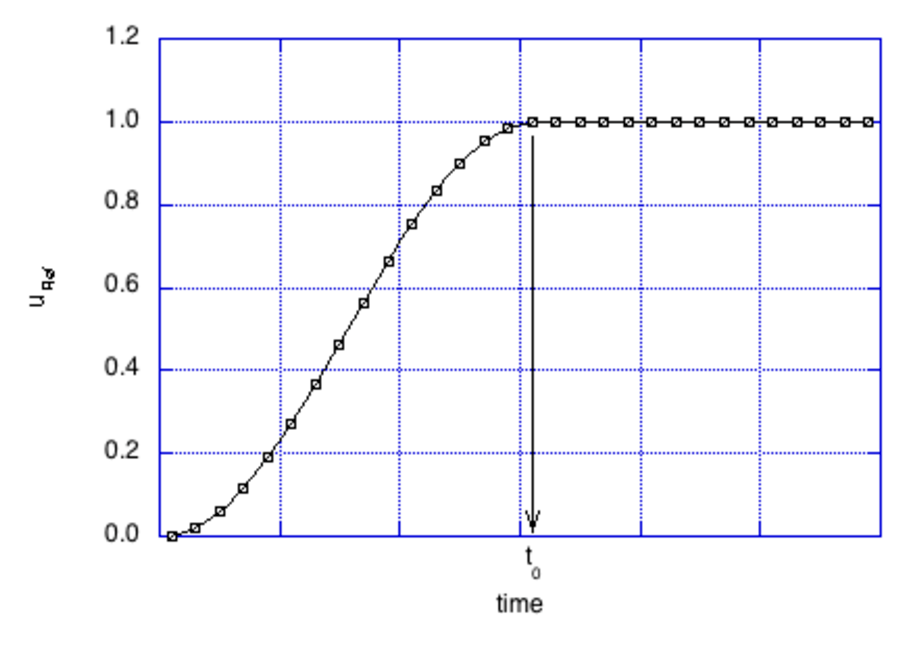
\includegraphics[width=7cm,clip]{accel_Velocity.eps}
\end{center}
\caption{加速中の速度プロファイル}
\label{fig:accel_velocity}
\end{figure}

%
\paragraph{時間積分幅$\Delta{t}$の指定}
\textbf{表\ref{tbl:delta t inc}}に時間積分幅\index{じかんせきぶんはば@時間積分幅}$\Delta{t}$の指定方法を示します.
拡散数\index{かくさんすう@拡散数}$D$は一次元の拡散方程式の場合$D=\alpha \delta t \slash h^2$で与えられます.$\alpha$は拡散係数で,Navier-Stokes方程式の場合$1/Re$,温度の輸送方程式の場合には$1/Pe$となります.安定性解析から$D<1 \slash 2$であることが要請されます.多次元の場合には,$d_m$を次元数として$\delta t<h^2 \slash (2d_m \alpha)$となります.

Delta\_tにはCFL数\index{CFL},または$\Delta t$を記述します.
時間積分幅の選択は,ソルバの種類を示すKind\_of\_Solverパラメータと関連があり,Solid\_Conductionの場合にはDt\_Directのみ選択できます.

\begin{table}[htdp]
\caption{Time\_Incrementのパラメータ指定}
\begin{center}
\small
\begin{tabular}{lll} \toprule
Dt\_Type & 時間積分幅の決定方法 & Delta\_tへの指定数値\\ \midrule
Direct & $\Delta t$を直接指定する & $\Delta t$\\
%CFL\_DFN\_MaxV & CFL\_MaxVと拡散数により制限される$\Delta t$の値の小さい方を選択\\
%CFL\_DFN\_RefV & CFL\_RefVと拡散数により制限される$\Delta t$の値の小さい方を選択\\
%CFL\_MaxV & CFL数を指定し,瞬時値の最大流速から$\Delta t$を決定 & CFL数\\
CFL\_Reference\_Velocity & CFL数を指定し,代表流速から$\Delta t$を決定 & CFL数\\
Diffusion & 拡散数から$\Delta t$を決定 & |\\
CFL\_Diffusion\_Reference\_Velocity & 代表流速に対するCFL数と拡散数から$\Delta t$を決定 & CFL数\\
%CFL\_MaxV\_CP & CFL数を指定し,音速を考慮した瞬時値の最大流速から$\Delta t$を決定 & CFL数\\
 \bottomrule
\end{tabular}
\end{center}
\label{tbl:delta t inc}
\end{table}

%
\pagebreak
\paragraph{計算時間の指定}
Period\_Typeで計算する時間の記述単位を指定します.
計算時間を時間で指定する場合,時間の単位は\hyperlink{tgt:unit}{Unit\_of\_Input\_Parameter}のモードに従います.
指定された単位の数値をCalculation\_Periodで指定します\footnote{SPHEREフレームワークでは,SPHERE定義要素としてCalculationStepsがありますが,内部的に上書きしています.}.

\end{indentation}



%%%
\pagebreak
\subsubsection{Treatment\_of\_Wall}

\hypertarget{tgt:treatment_of_wall}{壁面の扱い}について指定します.本パラメータは実験的実装です.

\begin{indentation}{3zw}{0zw}

{\small
\begin{program}
<Elem name="Treatment_of_Wall">
  <Param name="Pressure_Gradient" dtype="string" value="grad_zero"/>
  <Param name="Velocity_Profile"  dtype="string" value="no_slip"/>
</Elem>
\end{program}
}

各パラメータの意味について,\textbf{表\ref{tbl:wall_treatment}}に示します.
圧力勾配は法線方向の圧力勾配ゼロとNavier-Stokes方程式の圧力項を評価する2つの扱いが選択できます\footnote{現時点では,圧力勾配ゼロのみが選択できます.}.
速度プロファイルについては,滑りなし条件と壁関数を用いた近似が選択できます.壁関数は対数則が実装されています.詳細はCBCソルバークラス説明書をご覧ください\footnote{\today 未リリース.}.

\begin{table}[htdp]
\caption{壁面条件の指定}
\begin{center}
\small
\begin{tabular}{lll} \toprule
タグ & パラメータの値 & 説明\\ \midrule
Pressure\_Gradient & Grad\_Zero & 圧力勾配ゼロ\\
 & Grad\_NS & Navier-Stokes方程式から計算する\\ \hline
Velocity\_Profile  & No\_Slip & 滑りなし壁面条件\\
 & Slip & 滑り壁条件\\
 & Law\_of\_Wall & 壁法則\\ \bottomrule
\end{tabular}
\end{center}
\label{tbl:wall_treatment}
\end{table}

\end{indentation}


%%%
\pagebreak
\subsubsection{Unit}
\label{sec:p_unit}

入力ファイルと出力ファイルで用いる\hypertarget{tgt:unit}{単位を指定}します.

\begin{indentation}{3zw}{0zw}

{\small
\begin{program}
<Elem name="Unit">
  <Param name="Unit_of_Input_Parameter" dtype="STRING"  value="Dimensional" />
  <Param name="Pressure"                dtype="STRING"  value="gauge" />
  <Param name="Temperature"             dtype="STRING"  value="Celsius" />
</Elem>
\end{program}
}

各タグは,\textbf{表\ref{tbl:param_unit}}に示す単位の指定に用いられます.
有次元のファイル出力時には,圧力単位としてゲージ圧(Gauge Pressure)と絶対圧力(Absolute Pressure)が選択できます.
\textbf{式(\ref{eq:gauge pressure})}に示すゲージ圧を\textbf{式(\ref{eq:ND gauge})}により無次元化する場合に,基準圧として$p_0^\prime\,=\,1.0325\times 10^5$ [Pa]を用い,動圧が$10^0 \sim 10^3$程度とすると,$p \sim \mathrm{O}(1)$程度となるので,単精度計算では4桁程度有効桁が失われる場合もあります.
そのような場合,有次元値のファイル出力単位としてゲージ圧$p_g^\prime$を用います(非圧縮流れの場合には圧力差が意味をもつので,ゲージ圧でもかまいません).
ゲージ圧の基準となる大気圧$p_0^\prime\,$[Pa]は\hyperlink{tgt:reference}{Base\_Pressure}で指定します.
圧力単位の指定は,履歴ファイルのモニタ値にも適用されます.

\begin{equation}
p_g^\prime \,=\, p^\prime \,-\, p_0^\prime
\label{eq:gauge pressure}
\end{equation}

\begin{equation}
p \,=\, \frac{p_g^\prime}{\rho^\prime {u_0^\prime}^2}
\label{eq:ND gauge}
\end{equation}

\begin{table}[htdp]
\caption{単位の指定}
\begin{center}
\small
\begin{tabular}{lll} \toprule
タグ & 指定パラメータ & 説明\\ \midrule
Unit\_of\_Input\_Parameter & Dimensional or Non\_Dimensional & 入力パラメータファイルの単位を指定します(*1)\\
Pressure & Gauge or Absolute & 入力パラメータの単位が有次元のときに有効となります\\
Temperature & Celsius or Kelvin & 入力パラメータの単位が有次元のときに有効となります\\\bottomrule
\end{tabular}
\end{center}
\label{tbl:param_unit}
\end{table}

\end{indentation}



%%%
\pagebreak
\subsubsection{Version\_Info}

CBCソルバークラスとFlowBaseクラスの\hypertarget{tgt:version}{バージョン番号}を指定します.
異なる番号を指定している場合には,修正すべきバージョン番号が表示されるのでXMLファイルを変更します.

\begin{indentation}{3zw}{0zw}
\small
\begin{program}
<Elem name="Version_Info">
  <Param name="CBC"         dtype="INT"   value="127" />
  <Param name="Flow_Base"   dtype="INT"   value="225" />
</Elem>
\end{program}

\end{indentation}


%%%
\pagebreak
\subsubsection{VoxelDivisionMethod}
並列計算時の\hypertarget{tgt:voxel_division_method}{領域分割}をユーザーが明示的に指定します.直方体領域の計算空間を想定し,I, J, Kの各方向の分割数を指定します.
この指定が無い場合には,Sphereフレームワークがロードバランスが等しく,かつ通信面積が細小となる適切な分割を行います.

\begin{indentation}{3zw}{0zw}
\small
\begin{program}
<Elem name="VoxelDivisionMethod">
  <Param name="I"   dtype="INT"   value="8" />
  <Param name="J"   dtype="INT"   value="4" />
  <Param name="K"   dtype="INT"   value="5" />
</Elem>
\end{program}

\end{indentation}

%%% 隠しパラメータ
\begin{comment}
\subsubsection{Variable\_Range}

温度計算を実施する場合に,変数値を無次元値で[0,1]の範囲に\hypertarget{tgt:variable_range}{制限}することを指定します.

\begin{indentation}{3zw}{0zw}
\small

\begin{program}
<Param name="Variable_Range"     dtype="STRING" value="normal" />
\end{program}

\normalsize
温度の値に制限を課す場合に\textbf{表\ref{tbl:var_range}}に示すパラメータを使用します.保存則を満たさなくなるため,影響を考慮して利用してください.

\begin{table}[htdp]
\small
\caption{Variable\_Rangeのパラメータ指定}
\begin{center}
\begin{tabular}{ll} \toprule
タグ & モード\\ \midrule
cutoff & 値を無次元で[0, 1]に制限します\\
normal & 制限しません\\ \bottomrule
\end{tabular}
\end{center}
\label{tbl:var_range}
\end{table}

\end{indentation}
\end{comment}


%%%
\pagebreak
\subsection{Parameterセクション}
\label{sec:physical_parameter}

パラメータセクションでは,CBCソルバークラスの実行に必要な物理パラメータ\index{ぶつりぱらめーた@物理パラメータ}を記述します.



%%%
\subsubsection{Initial\_State}

\hypertarget{tgt:initial_state}{物理変数}の初期値\index{しょきち@初期値}を指定します.

\begin{indentation}{3zw}{0zw}

{\small
\begin{program}
<Elem name="Initial_State">
  <Param name="Density"     dtype="REAL" value="1.25e00" />
  <Param name="Pressure"    dtype="REAL" value="0.0" />
  <Param name="Temperature" dtype="REAL" value="20.0" />
  <Elem name="Velocity">
    <Param name="u" dtype="REAL" value="0.0"/>
    <Param name="v" dtype="REAL" value="0.0"/>
    <Param name="w" dtype="REAL" value="0.0"/>
  </Elem>
</Elem>
\end{program}
}

記述する初期値は有次元量で指定しますが,Solver\_Propertyセクションで\hyperlink{tgt:solver_property}{Kind\_of\_Solver}=\lq\lq Flow\_Only\rq\rq を指定した場合のみ,無次元での指定も可能です.
圧力値は,\hyperlink{tgt:unit}{Unit}で指定する圧力の単位に従います.
各変数の無次元化は以下のようになり,添え字の0は代表値または基準値を意味します.

\begin{equation}
\left.
\begin{array}{l}
\vspace{2mm}
\displaystyle{ \rho \,=\, \frac{\rho^{\prime}}{\rho_{0}^{\prime}} } \\
\vspace{2mm}
\displaystyle{ p \,=\, \frac{p^{\prime}-p_{0}^{\prime}}{\rho_{0}^{\prime}\,{u_{0}^{\prime}}^{2}} } \\
\vspace{2mm}
\displaystyle{ u_{i} \,=\, \frac{u_{i}^{\prime}}{u_0^{\prime}} } \\
\vspace{2mm}
\displaystyle{ \theta \,=\, \frac{\theta^{\prime}-\theta_{0}^{\prime}}{\Delta \theta^{\prime}} } 
\end{array} \qquad \right \}
\end{equation}

\end{indentation}

\vspace{3mm}
%%%
\subsubsection{Init\_Temp\_of\_Medium}
温度計算の場合に,割り当てた\hypertarget{tgt:initial_temp}{媒質}に対して初期温度を設定します.
媒質IDと流体・固体の種別は\hyperlink{tgt:model_setting}{Model\_Setting}と一致している必要があります.

{\small
\begin{program}
<Elem name="Init_Temp_of_Medium">
  <Param name="fluid" id="1"   dtype="real" value="20.0" />
  <Param name="solid" id="2"   dtype="real" value="34.0" />
  <Param name="solid" id="6"   dtype="real" value="34.0" />
  <Param name="solid" id="3"   dtype="real" value="35.0" />
  <Param name="fluid" id="4"   dtype="real" value="20.0" />
  <Param name="fluid" id="5"   dtype="real" value="20.0" />
  <Param name="fluid" id="10"  dtype="real" value="20.0" />
</Elem>
\end{program}
}

%%%
\pagebreak
\subsubsection{Intrinsic\_Example}

\hypertarget{tgt:intrinsic_example}{組み込み}例題\index{くみこみれいだい@組み込み例題}に固有のパラメータを指定します.

\begin{indentation}{3zw}{0zw}
\small

\begin{program}
<Elem name="Intrinsic_Example">
  ...
</Elem>
\end{program}

\normalsize
指定可能なパラメータは,\textbf{表\ref{tbl:intrinsic_parameter}}に示すように各\hyperlink{tgt:example}{組み込み例題}ごとに異なります.

\begin{table}[htdp]
\caption{Intrinsic\_Exampleセクションで指定できるパラメータ}
\begin{center}
\small
\begin{tabular}{llll} \toprule
組み込み例題 & 指定パラメータタグ & dtype & 指定値\\ \midrule
Duct3D & Shape     & STRING & Circular, Rectangular\\
       & Diameter  & REAL   & 断面径 [m]\\
       & Direction & STRING & X\_minus $|$ X\_plus $|$ Y\_minus $|$ Y\_plus $|$ Z\_minus $|$ Z\_plus\\
       & Driver    & REAL   & ドライバ部分の長さ [m]\\ \bottomrule
\end{tabular}
\end{center}
\label{tbl:intrinsic_parameter}
\end{table}

\end{indentation}



%%%
\pagebreak
\subsubsection{Reference}

解析に用いる無次元化の\hypertarget{tgt:reference}{基準量},あるいは無次元パラメータを指定します.

\begin{indentation}{3zw}{0zw}

{\small
\begin{program}
<Elem name="Reference">
  <Param name="Length"        dtype="REAL" value="1.0" />
  <Param name="Velocity"      dtype="REAL" value="1.0" />
  <Param name="Base_Pressure" dtype="REAL" value="101325" />
  <Param name="Gravity"       dtype="REAL" value="9.8" />
  <Param name="Reynolds"      dtype="REAL" value="1000.0" />
  <Param name="Prandtl"       dtype="REAL" value="0.71" />
  <Param name="Ref_ID"        dtype="INT"  value="1" />
</Elem>
\end{program}
}

\noindent \textbf{表\ref{tbl:ref_value}}に示すように基準量を必要に応じて記述できます.
無次元パラメータであるReynolds数とPrandtl数は,\hyperlink{tgt:unit}{Unit}の指定が無次元のときのみ指定できます.
Ref\_IDで指定するIDは,ボクセルモデル内で使われ,かつ\hyperlink{tgt:model_setting}{Model\_Setting}セクションで記述されている必要があります.固体熱伝導解析の場合には固体のIDを指定し,それ以外の(熱)流動解析の場合には流体のIDを指定します.

\begin{table}[htdp]
\caption{Referenceセクションで指定できるパラメータ}
\begin{center}
\small
\begin{tabular}{llll} \toprule
値 & 意味 & 単位\\ \midrule
Length & 代表長さ & $m$ &\\
Velocity & 代表速度 & $m/s$ &\\
Base\_Pressure & 基準圧力 & $Pa$ &\\
Gravity & 重力加速度 & $m^2/s$ &\\
%Grashof & グラショフ数 & |\\
Prandtl & プラントル数 & | & 無次元のときのみ指定\\
%Rayleigh & レイリー数 & |\\
Reynolds & レイノルズ数 & | & 無次元のときのみ指定\\
Ref\_ID & 代表物性値として指定する媒質ID & | &\\ \bottomrule
\end{tabular}
\end{center}
\label{tbl:ref_value}
\end{table}

\end{indentation}



%%%
\pagebreak
\subsubsection{Temperature}

\hypertarget{tgt:temperature}{温度計算}を実施する場合の基準量を有次元値で指定します.

\begin{indentation}{3zw}{0zw}

{\small
\begin{program}
<Elem name="Temperature">
  <Param name="Base"       dtype="REAL"   value="293.15" />
  <Param name="Difference" dtype="REAL"   value="35.0" />
</Elem>
\end{program}
}

基準温度(Base)と温度差(Difference)は,非圧縮計算のパッシブスカラーによる温度計算では温度場を特徴づける代表量となります.
単位は\hyperlink{tgt:unit}{Temperature}タグで指定します.

\end{indentation}



%%%
\pagebreak
\subsection{Medium\_Tableセクション}

ソルバーで利用する媒質の\hypertarget{tgt:medium_table}{物性値テーブル}を記述します.
ここで記述する媒質の基本リスト\index{きほんりすと@基本リスト!ばいしつの@媒質の---}は,解析に利用される候補です.
媒質は流体と固体が記述でき,\textbf{表\ref{tbl:MTLentry}}により媒質を指定します.

\begin{indentation}{3zw}{0zw}

{\small
\begin{program}
<Medium_Table>
  <Elem name="Fluid" id="100" comment="Air">
    <Param name="density"              dtype="REAL" value="1.1763" />
    <Param name="specific_heat"        dtype="REAL" value="1007" />
    <Param name="thermal_conductivity" dtype="REAL" value="2.614e-02" />
    <Param name="kinematic_viscosity"  dtype="REAL" value="15.83e-06" />
    <Param name="viscosity"            dtype="REAL" value="18.62e-06" />
    <Param name="sound_of_speed"       dtype="REAL" value="340.0" />
    <Param name="volume_expansion"     dtype="REAL" value="0.04e-3" />
  </Elem>
  <Elem name="Solid" id="600" comment="Fe">
    <Param name="density"              dtype="REAL" value="7870.0" />
    <Param name="specific_heat"        dtype="REAL" value="442.0" />
    <Param name="thermal_conductivity" dtype="REAL" value="80.3" />
  </Elem>
</Medium_Table>
\end{program}
}

\begin{table}[htdp]
\caption{Medium\_Tableに記述するパラメータ}
\begin{center}
\begin{tabular}{ll} \toprule
タグ & 説明\\ \midrule
Elem name & Fluid または Solid\\
ID & 媒質ID\\
comment & 媒質名\\ \bottomrule
\end{tabular}
\end{center}
\label{tbl:MTLentry}
\end{table}


各媒質は固体と流体によって記述しなければならない物性値が異なります.
指定できる項目を\textbf{表\ref{tbl:medium_tbl}}に示します.
固体については,密度・比熱・熱伝導率のみの記述となります.
各媒質の情報は,任意に指定するID番号によって管理されます.

\begin{table}[htdp]
\caption{Medium\_Tableにおける物性値の指定}
\begin{minipage}{.45\textwidth}
\begin{center}
\begin{tabular}{lll}\\ \toprule
Fluidのキーワード & 説明 & 単位\\ \midrule
Density & 密度 & $kg/m^3$\\
Specific\_Heat & 定圧比熱 & $kJ/(kg K)$\\
Thermal\_Conductivity & 熱伝導率 & $W/(m K)$\\
Kinematic\_Viscosity & 動粘性係数 & $m^2/s$\\
Viscosity & 粘性係数 & $Pa\,s$\\
Sound\_of\_Speed & 音速 & $m/s$\\
Volume\_Expansion & 体膨張率 & $1/K$\\ \bottomrule
\end{tabular}
\end{center}
\end{minipage} \hfill
\begin{minipage}{.45\textwidth}
\begin{center}
\begin{tabular}{lll}\\ \toprule
Solidのキーワード & 説明 & 単位\\ \midrule
Density & 密度 & $kg/m^3$\\
Specific\_Heat & 定圧比熱 & $kJ/(kg K)$\\
Thermal\_Conductivity & 熱伝導率 & $W/(m K)$\\ \bottomrule
\end{tabular}
\end{center}
\end{minipage}
\label{tbl:medium_tbl}
\end{table}

\end{indentation}





%%%
\chapter{境界条件}
\label{chpt:BC}
\begin{abstract}
本章では,CBCソルバークラスで設定できる境界条件の設定について説明します.
まず境界条件と媒質を指定するXMLタグの構造について述べた後,流れと熱の境界条件について説明します.
\end{abstract}
%
\include{CBC_BC}
%



%%%
\chapter{モニタリング機能}
\label{chpt:monitor}
\begin{abstract}
CBCソルバークラスには,計算中の任意点の物理量をモニターする仕組みがあります.本章では,その指定方法について説明します.
\end{abstract}
%
\include{CBC_monitor}

%\chapter{パラメータ入力}
%\label{chpt:vxpit}
%\include{CBC_vxpit}



%%%
\chapter{ソルバーの実行}
\label{chpt:solver}
\begin{abstract}
CBCソルバークラスの実行方法と出力ファイルについて説明します.
\end{abstract}
%
\include{CBC_Execution}



%%%
\chapter{アップデート情報}
\label{chpt:update}
\begin{abstract}
本ユーザガイドのアップデート情報について記します.
\end{abstract}
%
%\section{Update}
{ \small

%
\subparagraph{Version 1.1.9\hspace{1cm}2011/11/7}

\begin{description}
\begin{indentation}{3zw}{0zw}
\item[-] {}~\hyperlink{tgt:average_option}{時間平均パラメータ}の記述を修正しました.
\end{indentation}
\end{description}

\vspace{3mm}

%
\subparagraph{Version 1.1.8\hspace{1cm}2011/9/19}

\begin{description}
\begin{indentation}{3zw}{0zw}
\item[-] 距離情報を用いたスキームの導入に伴い,\hyperlink{tgt:solver_property}{形状近似度}と\hyperlink{tgt:intrinsic model}{IP\_Polygon}のパラメータを追加しました.
\end{indentation}
\end{description}

\vspace{3mm}

%
\subparagraph{Version 1.1.7\hspace{1cm}2011/9/6}

\begin{description}
\begin{indentation}{3zw}{0zw}
\item[-] 表\ref{tbl:intrinsic problems}のPPLT2DのキーワードをParallel\_Plate\_2Dに変更しました.
\item[-] 組み込みモデルのIOP\_Ductクラスの説明を追加しました.
\end{indentation}
\end{description}

\vspace{3mm}

%
\subparagraph{Version 1.1.6\hspace{1cm}2011/9/5}

\begin{description}
\begin{indentation}{3zw}{0zw}
\item[-] 組み込みモデルにCYLINDER, STEPクラスを追加しました.
\end{indentation}
\end{description}

\vspace{3mm}

%
\subparagraph{Version 1.1.5\hspace{1cm}2011/8/31}

\begin{description}
\begin{indentation}{3zw}{0zw}
\item[-] 組み込み例題を\hyperlink{tgt:intrinsic model}{組み込みモデル}として再編集し,\ref{chpt:solver}章の一部の内容を統合しました.
\item[-] 組み込みモデルにPPLT2Dクラスの説明を追加しました.
\end{indentation}
\end{description}

\vspace{3mm}

%
\subparagraph{Version 1.1.4\hspace{1cm}2011/7/28}

\begin{description}
\begin{indentation}{3zw}{0zw}
\item[-] 温度計算時,各媒質に対して\hyperlink{tgt:initial_temp}{初期温度を指定}できるようにしました.
\end{indentation}
\end{description}

\vspace{3mm}

%
\subparagraph{Version 1.1.3\hspace{1cm}2011/7/21}

\begin{description}
\begin{indentation}{3zw}{0zw}
\item[-] 外部領域面の流出境界条件を修正しました.
\end{indentation}
\end{description}

\vspace{3mm}

%
\subparagraph{Version 1.1.2\hspace{1cm}2011/7/11}

\begin{description}
\begin{indentation}{3zw}{0zw}
\item[-] automakeの環境が異なる場合の対応を追記しました.
\item[-] V-Sphereの倍精度と並列モジュールのオプション記述を追加しました.
\item[-] モデル作成に媒質数の制限について加筆しました.
\end{indentation}
\end{description}

\vspace{3mm}

%
\subparagraph{Version 1.1.1\hspace{1cm}2011/7/9}

\begin{description}
\begin{indentation}{3zw}{0zw}
\item[-] CBC Ver. 1.3.6対応
\item[-] 内部境界条件の設定方法を固体セルをキーIDとする方法に変更しました.
\end{indentation}
\end{description}

\vspace{3mm}

%
\subparagraph{Version 1.1.0\hspace{1cm}2011/6/30}

\begin{description}
\begin{indentation}{3zw}{0zw}
\item[-] 外部境界条件と内部境界条件の\hyperlink{tgt:BC policy}{ポリシ}を明示しました.
\item[-] 内部境界条件の注意事項を追記しました.
\end{indentation}
\end{description}

\vspace{3mm}

%
\subparagraph{Version 1.0.9\hspace{1cm}2011/6/21}

\begin{description}
\begin{indentation}{3zw}{0zw}
\item[-] 体裁を変更しました.
\item[-] インストールの章に,\hyperlink{tgt:win_compile}{Windows}でのコンパイルと\hyperlink{tgt:win_opmi_binary}{OpenMPIバイナリパッケージ}を用いたコンパイルを追記しました.
\item[-] 熱境界条件について,\hyperlink{tgt:spec of heat bc}{指定方法}のポリシを追加しました.
\end{indentation}
\end{description}

\vspace{3mm}

%
\subparagraph{Version 1.0.8\hspace{1cm}2011/6/8}

\begin{description}
\begin{indentation}{3zw}{0zw}
\item[-] 境界条件のセクションの構成を変更しました.
\item[-] 熱境界条件を加筆しました.
\end{indentation}
\end{description}

\vspace{3mm}

%
\subparagraph{Version 1.0.7\hspace{1cm}2011/4/11}

\begin{description}
\begin{indentation}{3zw}{0zw}
\item[-] 組み込み例題クラスの\hyperlink{tgt:intrinsic model}{解析モデル}を追記しました.
\end{indentation}
\end{description}

\vspace{3mm}

%
\subparagraph{Version 1.0.6\hspace{1cm}2011/2/11}

\begin{description}
\begin{indentation}{3zw}{0zw}
\item[-] サンプリングのファイル指定を\hyperlink{tgt:monitor_list}{Monitor\_List}に移動しました.
\end{indentation}
\end{description}

\vspace{3mm}

%
\subparagraph{Version 1.0.5\hspace{1cm}2011/1/6}

\begin{description}
\begin{indentation}{3zw}{0zw}
\item[-] 時間平均操作\hyperlink{tgt:average_option}{Average\_Option}のXMLパラメータ書式を変更しました.
\item[-] ファイル入出力\hyperlink{tgt:fileio}{File\_IO}のXMLパラメータ書式を変更しました.
\item[-] 入力ファイル\hyperlink{tgt:input_data}{InputData}のXMLパラメータ書式を変更しました.
\item[-] インターバルのXMLパラメータ指定をFile\_IOとLogセクションに移動しました.
\item[-] 反復パラメータ\hyperlink{tgt:iteration}{Iteration}に温度の反復パラメータを追加しました.
\item[-] ログ出力\hyperlink{tgt:log}{Log}のXMLパラメータ書式を変更しました.
\item[-] モニター指定\hyperlink{tgt:monitor_list}{Monitor\_List}のXMLパラメータ書式を変更しました.
\item[-] 時間制御指定\hyperlink{tgt:time_control}{Time\_Control}のXMLパラメータ書式を変更しました.
\item[-] 単位指定\hyperlink{tgt:unit}{Unit}のXMLパラメータ書式を変更しました.
\item[-] 第\ref{chpt:BC}章の境界条件を変更しました.
\item[-] 第\ref{chpt:monitor}章のXMLパラメータ書式を変更しました.
\item[-] 第\ref{chpt:solver}章を変更しました.
\end{indentation}
\end{description}

\vspace{3mm}

%
\subparagraph{Version 1.0.4\hspace{1cm}2010/12/22}

\begin{description}
\begin{indentation}{3zw}{0zw}
\item[-] パラメータ\hyperlink{tgt:external forcce}{外力項を用いた境界条件}を追加しました.
\item[-] 例題にSHC1Dを追加しました.
\item[-] 解法\hyperlink{tgt:algorithm}{アルゴリズム}に温度の陽解法と陰解法を追加,関連する変更を\hyperlink{tgt:iteration}{Iteration}にも行いました.
\item[-] 対流項スキームの\hyperlink{tgt:convection_term}{O3\_MUSCL}選択時に,minmodリミターを追加しました.
\item[-] ファイル出力指定に\hyperlink{tgt:fileio}{Debug\_Divergence}を追加しました.
\item[-] 内部境界に\hyperlink{tgt:inactive}{不活性境界条件}を追加しました.
\item[-] バージョン情報\hyperlink{tgt:version}{Version\_Info}の記述を変更しました.
\item[-] 分割方法について,\hypertarget{tgt:voxel_division}{VoxelDivisionMethod}を加筆しました.
\item[-] 第\ref{chpt:monitor}章のモニタリング機能を追加しました.また,\hyperlink{tgt:monitor_list}{Monitor\_List}を修正しました.
\end{indentation}
\end{description}

\vspace{3mm}

%
\subparagraph{Version 1.0.3\hspace{1cm}2010/12/7}

\begin{description}
\begin{indentation}{3zw}{0zw}
\item[-] 対流項指定のパラメータ\hyperlink{tgt:convection_term}{Convection\_Term}にO2\_Centralを追加しました.
\item[-] 組み込み例題に\hyperlink{tgt:example}{固体熱伝導}(SHC1D)を追加しました.
\item[-] ログ出力\hyperlink{tgt:log}{Log}で,性能プロファイリング出力に詳細レベルを追加しました.
\item[-] 出力ファイル\hyperlink{tgt:output_data}{OutputData}とログ出力\hyperlink{tgt:log}{Log}に壁面情報出力を追加しました.また,出力ファイルの種類を追加しました.
\item[-] Solver\_Propertyにおいて,\hyperlink{tgt:solver_property}{PDE\_type}の表を追加しました.また,定常/非定常の種別のキーワードをTime\_Variationに変更しました.
\item[-] 並列計算時のボクセル分割の指定方法\hyperlink{tgt:voxel_division}{VoxelDivisionMethod}の説明を追加しました.
\item[-] 外部境界条件の指定方法を変更しました.
\end{indentation}
\end{description}

\vspace{3mm}

%
\subparagraph{Version 1.0.2\hspace{1cm}2010/11/16}

\begin{description}
\begin{indentation}{3zw}{0zw}
\item[-] V-Sphere 1.8.2に対応
\item[-] パラメータInterval,\hyperlink{tgt:log}{Log},\hyperlink{tgt:reference_frame}{Reference\_Frame},\hyperlink{tgt:time_control}{Time\_Control}の指定方法を変更しました.
\item[-] パラメータ\hyperlink{tgt:iteration}{Iteration},\hyperlink{tgt:version}{Version}の表記を修正しました.
\item[-] 境界条件\hyperlink{tgt:preriodic}{周期境界}の指定方法を変更しました.
\end{indentation}
\end{description}

\vspace{3mm}

%
\subparagraph{Version 1.0.1\hspace{1cm}2010/11/1}

\begin{description}
\begin{indentation}{3zw}{0zw}
\item[-] パラメータに\hyperlink{tgt:log}{Log}の説明を追記しました.
\item[-] パラメータの\hyperlink{tgt:interval}{Interval}と\hyperlink{tgt:time_control}{Time\_Control}の時刻指定について,StepとTimeによる指定を排他的にしました.
\item[-] CBCソルバークラスの\hyperlink{tgt:installCBC}{インストール}のセクションで,ディレクトリ構成の変更とdoxygenファイルについて追記しました.
\end{indentation}
\end{description}

\vspace{3mm}

%
\subparagraph{Version 1.0.0\hspace{1cm}2010/10/9}

\begin{description}
\begin{indentation}{3zw}{0zw}
\item[-] ユーザガイド(本編:cbc\_UG.pdf)と内部情報(Inside\_CBC.pdf)を分離しました.
\end{indentation}
\end{description}

} % end of small


%
\bibliographystyle{junsrt}
\bibliography{cbc_UG}

\newpage
\printindex
%
%
\end{document}